\documentclass[12pt,a4paper]{article}
\usepackage[a4paper, margin=0.8in, headheight=14pt]{geometry}
\usepackage{fontspec}
\usepackage{unicode-math}
\setmainfont{TeX Gyre Pagella}
\setmonofont[Scale=0.88]{TeX Gyre Cursor}
\setmathfont{Latin Modern Math}
\usepackage{xcolor}
\usepackage{colortbl}
\usepackage{titlesec}
\usepackage{enumitem}
\usepackage{tabularx}
\usepackage{booktabs}
\usepackage{array}
\usepackage{amsmath}
\usepackage{tikz}
\usetikzlibrary{shapes.geometric, arrows.meta, positioning, calc, fit, decorations.pathreplacing, decorations.pathmorphing, patterns, backgrounds}
\usepackage[american]{circuitikz}
\usepackage{tcolorbox}
\tcbuselibrary{skins, breakable}
\usepackage{etoolbox}
\usepackage{hyperref}
\usepackage{fancyhdr}
\usepackage{graphicx}
\usepackage{microtype}
\hyphenpenalty=10000
\exhyphenpenalty=10000
\sloppy
\usepackage{caption}
\usepackage{setspace}
\usepackage{multirow}
\usepackage{tocloft}
\newcommand{\Q}[1]{\textbf{#1}\par\noindent\ignorespaces}
\definecolor{myred}{RGB}{196,30,58}
\definecolor{mydark}{RGB}{30,30,50}
\definecolor{mygreen}{RGB}{14,120,80}
\definecolor{myteal}{RGB}{0,130,140}
\definecolor{myamber}{RGB}{180,100,0}
\definecolor{mypurple}{RGB}{100,30,160}
\definecolor{mygray}{RGB}{246,247,249}
\definecolor{mgframe}{RGB}{180,185,200}
\definecolor{watermark}{RGB}{145,150,170}
\definecolor{hdrred}{RGB}{250,232,235}
\definecolor{hdrgreen}{RGB}{220,244,233}
\definecolor{hdrteal}{RGB}{220,242,244}
\definecolor{hdramber}{RGB}{253,242,215}
\definecolor{hdrpurple}{RGB}{238,228,255}
\AfterEndEnvironment{tcolorbox}{\color{mydark}}

\titleformat{\section}{\large\bfseries\color{myred}}{\thesection.}{0.5em}{}[\vspace{1pt}{\color{myred}\rule{\linewidth}{0.8pt}}]
\titleformat{\subsection}{\normalsize\bfseries\color{myteal}}{\thesubsection}{0.5em}{}
\titlespacing*{\section}{0pt}{18pt}{7pt}
\titlespacing*{\subsection}{0pt}{11pt}{4pt}
\setlength{\parindent}{0pt}
\setlength{\parskip}{4pt}
\renewcommand{\cfttoctitlefont}{\large\bfseries\color{myred}}
\renewcommand{\cftaftertoctitle}{\par\noindent{\color{myred}\rule{\linewidth}{0.8pt}}}
\setlength{\cftbeforetoctitleskip}{0pt}
\setlength{\cftaftertoctitleskip}{6pt}
\renewcommand{\cftsecfont}{\normalsize\bfseries\color{mydark}}
\renewcommand{\cftsecpagefont}{\normalsize\bfseries\color{mydark}}
\renewcommand{\cftsecleader}{\cftdotfill{\cftdotsep}}
\setlength{\cftbeforesecskip}{7pt}
\renewcommand{\cftsubsecfont}{\small\color{mydark}}
\renewcommand{\cftsubsecpagefont}{\small\color{mydark}}
\setlength{\cftbeforesubsecskip}{3pt}
\setlength{\cftsubsecindent}{1.4em}
\renewcommand{\cftpartfont}{\normalsize\bfseries\color{myteal}}
\renewcommand{\cftpartpagefont}{\normalsize\bfseries\color{myteal}}
\setlength{\cftbeforepartskip}{14pt}
\renewcommand{\arraystretch}{1.45}
\setlength{\tabcolsep}{6pt}
\arrayrulecolor{mydark}
\newcolumntype{B}[1]{>{\small\bfseries\raggedright\arraybackslash}m{#1}}
\newcolumntype{C}[1]{>{\centering\arraybackslash}m{#1}}
\newcolumntype{Y}{>{\small\raggedright\arraybackslash}X}
\renewcommand{\tabularxcolumn}[1]{m{#1}}
\newcommand{\currmodule}{Module 1}
\pagestyle{fancy}
\fancyhf{}
\fancyhead[L]{\small\color{myred}\textbf{BS-PH101}\;\color{mydark}--- Physics-I}
\fancyhead[R]{\small\color{myteal}\textbf{\currmodule\ Notes}}
\fancyfoot[C]{\small\color{mydark}\thepage}
\fancyfoot[R]{\small\color{watermark}\textit{\copyright\ Biraj}}
\renewcommand{\headrulewidth}{0.5pt}
\renewcommand{\footrulewidth}{0.3pt}

\hypersetup{colorlinks=true, linkcolor=myteal, urlcolor=myteal,
  pdfauthor={Biraj Sarkar},
  pdftitle={BS-PH101 --- Combined Notes}}

\tcbset{
  tikzbox/.style={
    colback=mygray, colframe=mgframe, boxrule=0.6pt, arc=4pt,
    left=8pt, right=8pt, top=6pt, bottom=6pt,
    colbacktitle=mgframe, coltitle=mydark, fonttitle=\small\bfseries
  },
  defbox/.style={
    colback=hdrgreen, colframe=mygreen, boxrule=0.8pt, arc=4pt,
    left=9pt, right=9pt, top=6pt, bottom=6pt,
    colbacktitle=mygreen, coltitle=white, fonttitle=\small\bfseries
  },
  formulabox/.style={
    colback=hdrteal, colframe=myteal, boxrule=0.8pt, arc=4pt,
    left=9pt, right=9pt, top=7pt, bottom=7pt,
    colbacktitle=myteal, coltitle=white, fonttitle=\small\bfseries
  },
  examplebox/.style={
    colback=hdramber, colframe=myamber, boxrule=0.8pt, arc=4pt,
    left=9pt, right=9pt, top=6pt, bottom=6pt,
    colbacktitle=myamber, coltitle=white, fonttitle=\small\bfseries
  },
  masonbox/.style={
    colback=hdrpurple, colframe=mypurple, boxrule=0.8pt, arc=4pt,
    left=9pt, right=9pt, top=6pt, bottom=6pt,
    colbacktitle=mypurple, coltitle=white, fonttitle=\small\bfseries
  },
  exambox/.style={
    colback=hdrpurple, colframe=mypurple, boxrule=1pt, arc=5pt,
    left=10pt, right=10pt, top=8pt, bottom=8pt,
    colbacktitle=mypurple, coltitle=white, fonttitle=\bfseries,
    breakable, title after break={\textbf{Frequently Asked / Viva Questions (contd.)}}
  }
}
\tcbset{breakable}
\tcbset{coltext=mydark}
\tcbset{after={\color{mydark}}}

\tikzset{
  block/.style={rectangle, draw=myteal, fill=hdrteal, text width=2.4cm, align=center, minimum height=0.95cm, font=\small, rounded corners=3pt, line width=0.7pt},
  redblock/.style={rectangle, draw=myred, fill=hdrred, text width=2.4cm, align=center, minimum height=0.95cm, font=\small, rounded corners=3pt, line width=0.7pt},
  arrow/.style={-Stealth, thick, color=mydark},
  redarrow/.style={-Stealth, thick, color=myred},
  line/.style={thick, color=mydark}
}

\newcommand{\modulestart}[2]{%
  \clearpage
  \renewcommand{\currmodule}{Module #1}%
  \renewcommand{\theHsection}{mod#1.\arabic{section}}%
  \renewcommand{\theHsubsection}{\theHsection.\arabic{subsection}}%
  \renewcommand{\theHsubsubsection}{\theHsubsection.\arabic{subsubsection}}%
  \phantomsection
  \addcontentsline{toc}{part}{Module #1: #2}%
  \setcounter{section}{0}%
  \begin{center}
    \vspace*{1.0cm}
    {\Huge\bfseries\color{myred} Module #1}\\[10pt]
    {\Large\bfseries\color{mydark} #2}\\[10pt]
    {\color{myred}\rule{0.55\linewidth}{1.2pt}}
  \end{center}
  \vspace{14pt}
}
\begin{document}

\thispagestyle{empty}

% ─── Page Border (TikZ Overlay) ────────────────────────────────────────────────
\begin{tikzpicture}[remember picture, overlay]
  % Outer border (fine line in mgframe)
  \draw[color=mgframe, line width=1.5pt] 
    ($(current page.north west) + (0.6in, -0.6in)$) rectangle 
    ($(current page.south east) + (-0.6in, 0.6in)$);
  % Inner border (finer accent line in myred)
  \draw[color=myred, line width=0.8pt] 
    ($(current page.north west) + (0.65in, -0.65in)$) rectangle 
    ($(current page.south east) + (-0.65in, 0.65in)$);
\end{tikzpicture}

\vspace*{1.0cm}
\begin{center}
  {\Huge\bfseries\color{myred} BS-PH101}\\[10pt]
  {\LARGE\bfseries\color{mydark} Physics-I}\\[20pt]
  {\color{myred}\rule{0.7\linewidth}{1.5pt}}\\[18pt]
  {\Large\color{myteal}\textbf{Combined Module Notes}}\\[8pt]
  {\large\color{mydark} Modules 1 -- 5}\\[40pt]
  {\normalsize\color{mydark} Semester I/II \quad$\bullet$\quad ECE \quad$\bullet$\quad 4 Credits}\\[12pt]
  {\normalsize\color{mydark} CGEC \;$|$\; B.Tech ECE (2023--27)}
\end{center}
\vspace{1.0cm}
\begin{center}
  \begin{tcolorbox}[colback=mygray, colframe=mgframe, boxrule=0.5pt, arc=3pt, width=0.85\linewidth]
    \centering\small\color{mydark}
    \textbf{Disclaimer / Study Guide Notice:}\\
    These are condensed \textbf{Short Notes} focusing on core theory, key formulas, block/circuit diagrams, and standard viva Q\&As for university exam revision. Exhaustive numerical practice problems and derivation edge cases are not covered. This serves as a quick-revision reference guide for students.
  \end{tcolorbox}
\end{center}
\vfill
\vspace{0.6cm}
\begin{center}
  {\large\bfseries\color{mypurple} Biraj Sarkar}\\[16pt]
  {\footnotesize\color{watermark}\textbf{IN ASSOCIATION WITH}}\\[8pt]
  {\small\bfseries\color{mydark} MAKAUT Wingman \quad$\bullet$\quad MAKAUT Future Minds}\\[12pt]
  {\large\bfseries\color{myteal} Cooch Behar Government Engineering College}
\end{center}
\vfill
\begin{center}{\small\color{watermark}\textit{Exam-Ready Notes}}\end{center}
\clearpage

\hypersetup{linkcolor=mydark}
\tableofcontents
\hypersetup{linkcolor=myteal}
\clearpage

% -- Module 1 -----------------------------------------------------------------
\modulestart{1}{Constraints and Friction}

\section{Constraints and Friction}

\subsection{Constraints and Degrees of Freedom}

\begin{tcolorbox}[defbox, title={\textbf{Definition: Constraint and Degrees of Freedom}}]
A \textbf{constraint} is any physical restriction on the position or motion of a mechanical system. The number of independent coordinates required to completely specify the configuration of a system is called its \textbf{Degrees of Freedom (DOF)}.
\end{tcolorbox}

If a system consists of $N$ particles in 3D space subject to $k$ independent constraint equations, the number of degrees of freedom is given by:
\begin{equation}
f = 3N - k
\end{equation}

\textbf{Classification of Constraints:}\par\vspace{6pt}\noindent
\begin{tabularx}{\linewidth}{|B{3.2cm}|Y|Y|}
\hline
\textbf{Constraint Type} & \textbf{Condition / Mathematical Form} & \textbf{Physical Example} \\
\hline
\textbf{Holonomic} & Expressible as $f(r_1, r_2, \ldots, r_N, t) = 0$ (integrable algebraic relations). & Rigid body ($|\vec{r}_i - \vec{r}_j| = c$), simple pendulum ($r = L$). \\
\hline
\textbf{Non-Holonomic} & Expressible as inequalities or non-integrable differential relations ($f(\vec{r}, \dot{\vec{r}}, t) = 0$). & Rolling without slipping on a rough plane, gas molecules in a container ($r \le R$). \\
\hline
\textbf{Scleronomic} & Constraint equations do not explicitly depend on time $t$ ($\partial f / \partial t = 0$). & Bead on a fixed wire ring, rigid dumbbell. \\
\hline
\textbf{Rheonomic} & Constraint equations explicitly depend on time $t$ ($\partial f / \partial t \neq 0$). & Bead on a wire ring rotating with constant angular velocity $\omega$. \\
\hline
\end{tabularx}

\subsection{Friction and Laws of Friction}

Friction is the resistive contact force that opposes the relative motion or tendency of relative motion between two surfaces in contact.

\begin{tcolorbox}[formulabox, title={\textbf{Key Laws and Relations of Friction}}]
\begin{itemize}[leftmargin=*, itemsep=2pt]
  \item \textbf{Static Friction ($f_s$):} Self-adjusting force. Maximum value is limiting friction:
  \begin{equation}
  f_{s,\max} = \mu_s N
  \end{equation}
  \item \textbf{Kinetic Friction ($f_k$):} Constant resistive force during motion:
  \begin{equation}
  f_k = \mu_k N \quad (\text{where } \mu_k < \mu_s)
  \end{equation}
  \item \textbf{Angle of Friction ($\lambda$):} Angle between total contact reaction $\vec{R}$ and normal reaction $\vec{N}$:
  \begin{equation}
  \tan \lambda = \frac{f_{s,\max}}{N} = \mu_s \implies \lambda = \tan^{-1}(\mu_s)
  \end{equation}
  \item \textbf{Angle of Repose ($\theta_r$):} Maximum angle of inclination of a rough plane at which a body remains at rest without sliding:
  \begin{equation}
  m g \sin \theta_r = \mu_s m g \cos \theta_r \implies \tan \theta_r = \mu_s \implies \theta_r = \lambda
  \end{equation}
\end{itemize}
\end{tcolorbox}

\begin{tcolorbox}[examplebox, title={\textbf{Solved Problem 1: Block on an Inclined Plane with Friction}}]
\textbf{Problem:} A block of mass $m = 5\text{ kg}$ rests on an inclined plane of angle $\theta = 30^\circ$. The coefficient of static friction is $\mu_s = 0.4$. Determine whether the block slides down, and find the frictional force.

\textbf{Solution:}\par\noindent
\begin{enumerate}[leftmargin=*, itemsep=2pt]
  \item Component of gravity along the incline: $F_{\text{down}} = m g \sin 30^\circ = 5 \times 9.8 \times 0.5 = 24.5\text{ N}$.
  \item Normal reaction: $N = m g \cos 30^\circ = 5 \times 9.8 \times 0.866 = 42.435\text{ N}$.
  \item Maximum limiting static friction: $f_{s,\max} = \mu_s N = 0.4 \times 42.435 = 16.97\text{ N}$.
  \item Since $F_{\text{down}} (24.5\text{ N}) > f_{s,\max} (16.97\text{ N})$, the block \textbf{will slide down}. The friction force acting up the plane during motion is kinetic friction $f_k = \mu_k N$.
\end{enumerate}
\end{tcolorbox}

\begin{tcolorbox}[examplebox, title={\textbf{Solved Problem 2: Degrees of Freedom of Connected Bodies}}]
\textbf{Problem:} Find the degrees of freedom for: (a) A double pendulum moving in a plane, (b) Two particles connected by a rigid rod free to move in 3D space.

\textbf{Solution:}\par\noindent
\begin{enumerate}[leftmargin=*, itemsep=2pt]
  \item \textbf{Double Pendulum in 2D:} $N=2$ particles, constrained to plane ($z_1=0, z_2=0$), fixed length $r_1=L_1$ and $|\vec{r}_2-\vec{r}_1|=L_2$. Total independent angles $\theta_1, \theta_2$. Hence \textbf{$\text{DOF} = 2$}.
  \item \textbf{Rigid Dumbbell in 3D:} $N=2$ particles in 3D ($6$ coordinates) subject to $k=1$ constraint ($|\vec{r}_1 - \vec{r}_2| = d$). Hence $\text{DOF} = 3(2) - 1 = \mathbf{5}$ (3 translational, 2 rotational).
\end{enumerate}
\end{tcolorbox}

% =============================================================================
% SECTION 2: VECTOR CALCULUS & POTENTIAL ENERGY FUNCTION
% =============================================================================
\section{Vector Calculus and Potential Energy Function}

\subsection{Gradient, Divergence, and Curl}

\begin{tcolorbox}[defbox, title={\textbf{Definition: Gradient, Divergence, and Curl}}]
\begin{itemize}[leftmargin=*, itemsep=2pt]
  \item \textbf{Gradient ($\nabla V$):} Vector representing the rate and direction of maximum spatial change of a scalar field $V(x,y,z)$.
  \item \textbf{Divergence ($\nabla \cdot \vec{A}$):} Scalar representing the net outward flux of a vector field per unit volume.
  \item \textbf{Curl ($\nabla \times \vec{A}$):} Vector representing the circulation or rotational density of a vector field.
\end{itemize}
\end{tcolorbox}

\begin{tcolorbox}[formulabox, title={\textbf{Mathematical Definitions in Cartesian Coordinates}}]
\begin{align}
\text{grad } V = \nabla V &= \frac{\partial V}{\partial x}\hat{i} + \frac{\partial V}{\partial y}\hat{j} + \frac{\partial V}{\partial z}\hat{k} \\[4pt]
\text{div } \vec{A} = \nabla \cdot \vec{A} &= \frac{\partial A_x}{\partial x} + \frac{\partial A_y}{\partial y} + \frac{\partial A_z}{\partial z} \\[4pt]
\text{curl } \vec{A} = \nabla \times \vec{A} &= 
\begin{vmatrix}
\hat{i} & \hat{j} & \hat{k} \\
\frac{\partial}{\partial x} & \frac{\partial}{\partial y} & \frac{\partial}{\partial z} \\
A_x & A_y & A_z
\end{vmatrix}
\end{align}
\end{tcolorbox}

\subsection{\texorpdfstring{Potential Energy Function $F = -\text{grad } V$}{Potential Energy Function F = -grad V}}

For a conservative force field $\vec{F}$, the work done along a closed path is zero ($\oint \vec{F} \cdot d\vec{r} = 0$). This implies $\vec{F}$ can be expressed as the negative gradient of a scalar potential energy function $V(\vec{r})$:
\begin{equation}
\vec{F} = -\nabla V = -\left(\frac{\partial V}{\partial x}\hat{i} + \frac{\partial V}{\partial y}\hat{j} + \frac{\partial V}{\partial z}\hat{k}\right)
\end{equation}

\textbf{Physical Meaning of Negative Sign:} The force acts in the direction of \textit{decreasing} potential energy (towards stable equilibrium).

\textbf{Equipotential Surfaces:} A surface on which the potential energy $V(\vec{r}) = \text{constant}$.
\begin{itemize}[leftmargin=*, itemsep=2pt]
  \item Work done in moving a mass along an equipotential surface is zero: $dW = \vec{F} \cdot d\vec{r} = -dV = 0$.
  \item The force vector $\vec{F}$ is everywhere perpendicular to the equipotential surface passing through that point.
\end{itemize}

\begin{tcolorbox}[examplebox, title={\textbf{Solved Problem 3: Deriving Force from Potential Energy}}]
\textbf{Problem:} Given potential energy $V(x,y,z) = 3x^2 y - y^3 z^2$, calculate force $\vec{F}$ at point $(1, -1, 2)$.

\textbf{Solution:}\par\noindent
\begin{enumerate}[leftmargin=*, itemsep=2pt]
  \item Calculate partial derivatives:
   $\frac{\partial V}{\partial x} = 6x y$, \quad $\frac{\partial V}{\partial y} = 3x^2 - 3y^2 z^2$, \quad $\frac{\partial V}{\partial z} = -2y^3 z$.
  \item Evaluate at $(1, -1, 2)$:
   $\frac{\partial V}{\partial x} = 6(1)(-1) = -6$, \quad $\frac{\partial V}{\partial y} = 3(1)^2 - 3(-1)^2(2)^2 = 3 - 12 = -9$, \quad $\frac{\partial V}{\partial z} = -2(-1)^3(2) = 4$.
  \item Substitute into $\vec{F} = -\nabla V$:
   \begin{equation}
   \vec{F} = -(-6\hat{i} - 9\hat{j} + 4\hat{k}) = \mathbf{6\hat{i} + 9\hat{j} - 4\hat{k} \text{ N}}
   \end{equation}
\end{enumerate}
\end{tcolorbox}

% =============================================================================
% SECTION 3: CONSERVATION LAWS
% =============================================================================
\section{Conservative Forces and Conservation Laws}

\subsection{Conservative vs. Non-Conservative Forces}

\textbf{Comparative Breakdown:}\par\vspace{6pt}\noindent
\begin{tabularx}{\linewidth}{|B{3.5cm}|Y|Y|}
\hline
\textbf{Property} & \textbf{Conservative Force} & \textbf{Non-Conservative Force} \\
\hline
\textbf{Work Dependence} & Work done depends only on initial and final positions. & Work done depends on the actual path taken. \\
\hline
\textbf{Closed Path Work} & $\oint \vec{F} \cdot d\vec{r} = 0$. & $\oint \vec{F} \cdot d\vec{r} \neq 0$. \\
\hline
\textbf{Curl Condition} & $\nabla \times \vec{F} = 0$ (Irrotational). & $\nabla \times \vec{F} \neq 0$. \\
\hline
\textbf{Potential Energy} & Expressible as $\vec{F} = -\nabla V$. & Potential energy function cannot be defined. \\
\hline
\textbf{Mechanical Energy} & Total mechanical energy $(E = K + V)$ is conserved. & Mechanical energy is dissipated as heat/sound. \\
\hline
\textbf{Examples} & Gravitational force, Electrostatic force, Spring force. & Friction, Viscosity, Air resistance. \\
\hline
\end{tabularx}

\subsection{Fundamental Conservation Laws}

\begin{tcolorbox}[formulabox, title={\textbf{Conservation Theorems}}]
\begin{enumerate}[leftmargin=*, itemsep=4pt]
  \item \textbf{Conservation of Linear Momentum:} If net external force $\vec{F}_{\text{ext}} = 0$, then:
  \begin{equation}
  \frac{d\vec{P}}{dt} = 0 \implies \vec{P} = \sum m_i \vec{v}_i = \text{constant}
  \end{equation}
  \item \textbf{Conservation of Angular Momentum:} If net external torque $\vec{\tau}_{\text{ext}} = \vec{r} \times \vec{F}_{\text{ext}} = 0$, then:
  \begin{equation}
  \frac{d\vec{L}}{dt} = 0 \implies \vec{L} = \vec{r} \times \vec{P} = I\vec{\omega} = \text{constant}
  \end{equation}
  \item \textbf{Conservation of Energy:} In an isolated system with conservative forces:
  \begin{equation}
  E_{\text{total}} = K + V = \frac{1}{2} m v^2 + V(\vec{r}) = \text{constant}
  \end{equation}
\end{enumerate}
\end{tcolorbox}

% =============================================================================
% SECTION 4: NON-INERTIAL FRAMES & PSEUDO FORCES
% =============================================================================
\section{Non-Inertial Frames of Reference}

\subsection{Inertial vs. Non-Inertial Frames}

\begin{tcolorbox}[defbox, title={\textbf{Definition: Frames of Reference}}]
\begin{itemize}[leftmargin=*, itemsep=2pt]
  \item \textbf{Inertial Frame:} A frame of reference moving with zero acceleration (at rest or constant velocity) in which Newton's laws of motion hold strictly.
  \item \textbf{Non-Inertial Frame:} An accelerating or rotating frame of reference in which Newton's laws do not hold directly unless fictitious / pseudo forces are introduced.
\end{itemize}
\end{tcolorbox}

\subsection{Rotating Frames: Centrifugal and Coriolis Forces}

Consider a frame $S'$ rotating with constant angular velocity $\vec{\omega}$ relative to a stationary inertial frame $S$.

\begin{tcolorbox}[formulabox, title={\textbf{Transformation Equation for Acceleration}}]
The transformation relation between acceleration in fixed frame $\vec{a}_S$ and rotating frame $\vec{a}_{S'}$ is:
\begin{equation}
\vec{a}_S = \vec{a}_{S'} + 2(\vec{\omega} \times \vec{v}') + \vec{\omega} \times (\vec{\omega} \times \vec{r})
\end{equation}
Multiplying by mass $m$, the effective force in the rotating frame is:
\begin{equation}
\vec{F}' = m \vec{a}_{S'} = \vec{F}_{\text{real}} - \underbrace{2m(\vec{\omega} \times \vec{v}')}_{\text{Coriolis Force } \vec{F}_{\text{cor}}} - \underbrace{m\vec{\omega} \times (\vec{\omega} \times \vec{r})}_{\text{Centrifugal Force } \vec{F}_{\text{cent}}}
\end{equation}
\end{tcolorbox}

\textbf{Properties of Rotating Fictitious Forces:}\par\vspace{6pt}\noindent
\begin{tabularx}{\linewidth}{|B{3.2cm}|Y|Y|}
\hline
\textbf{Force} & \textbf{Vector Expression} & \textbf{Key Characteristics} \\
\hline
\textbf{Centrifugal Force} & $\vec{F}_{\text{cent}} = -m\vec{\omega} \times (\vec{\omega} \times \vec{r}) = m \omega^2 r_{\perp} \hat{r}$ & Directed radially outward from axis of rotation. Present even if particle is stationary in rotating frame ($\vec{v}' = 0$). \\
\hline
\textbf{Coriolis Force} & $\vec{F}_{\text{cor}} = -2m(\vec{\omega} \times \vec{v}')$ & Perpendicular to both velocity $\vec{v}'$ and angular velocity $\vec{\omega}$. Acts only when particle is in motion ($\vec{v}' \neq 0$). Does zero work ($W = 0$). \\
\hline
\end{tabularx}

\textbf{Physical Effects of Coriolis Force on Earth:}
\begin{itemize}[leftmargin=*, itemsep=2pt]
  \item \textbf{Deflection of Moving Objects:} Moving bodies in Northern Hemisphere are deflected to their \textit{right}, while in Southern Hemisphere to their \textit{left} (causes cyclone rotation direction).
  \item \textbf{Eastward Deflection of Freely Falling Body:} A body dropped from height $h$ at latitude $\lambda$ experiences an eastward deflection $\Delta x = \frac{1}{3} \omega g \cos \lambda \sqrt{\frac{8h^3}{g}}$.
  \item \textbf{Foucault Pendulum:} Demonstrates Earth's rotation directly via precession of its oscillation plane at angular rate $\Omega = \omega \sin \lambda$.
\end{itemize}

\begin{tcolorbox}[examplebox, title={\textbf{Solved Problem 4: Eastward Deflection Calculation}}]
\textbf{Problem:} Calculate the eastward deflection due to Coriolis force for a body dropped from a height $h = 100\text{ m}$ at Kolkata (latitude $\lambda = 22.5^\circ\text{N}$). (Take $\omega = 7.29 \times 10^{-5}\text{ rad/s}, g = 9.8\text{ m/s}^2$).

\textbf{Solution:}\par\noindent
\begin{enumerate}[leftmargin=*, itemsep=2pt]
  \item Formula for eastward deflection:
   \begin{equation}
   d = \frac{1}{3} \omega g \cos\lambda \sqrt{\frac{8 h^3}{g}}
   \end{equation}
  \item Calculate time of fall: $t = \sqrt{\frac{2h}{g}} = \sqrt{\frac{200}{9.8}} = 4.518\text{ s}$.
  \item Substitute values:
   $d = \frac{1}{3} (7.29 \times 10^{-5}) (9.8) \cos(22.5^\circ) (4.518)^3$
   $\cos 22.5^\circ = 0.9239$, \quad $(4.518)^3 = 92.23$.
   $d = 0.333 \times 7.29 \times 10^{-5} \times 9.8 \times 0.9239 \times 92.23 = \mathbf{0.0195\text{ m} = 1.95\text{ cm}}$.
\end{enumerate}
\end{tcolorbox}

% =============================================================================
% SECTION 5: HARMONIC OSCILLATORS
% =============================================================================
\section{Harmonic Oscillations}

\subsection{Damped Harmonic Motion}

When an oscillator experiences a viscous damping force proportional to velocity ($F_{\text{damping}} = -b \dot{x}$), the equation of motion is:
\begin{equation}
m \ddot{x} + b \dot{x} + k x = 0 \implies \ddot{x} + 2\gamma \dot{x} + \omega_0^2 x = 0
\end{equation}
where $\gamma = \frac{b}{2m}$ is the damping coefficient and $\omega_0 = \sqrt{\frac{k}{m}}$ is the natural frequency.

Assuming solution $x(t) = C e^{r t}$, the roots of characteristic equation are $r = -\gamma \pm \sqrt{\gamma^2 - \omega_0^2}$.

\begin{tcolorbox}[formulabox, title={\textbf{Three Cases of Damped Motion}}]
\begin{enumerate}[leftmargin=*, itemsep=4pt]
  \item \textbf{Overdamped ($\gamma > \omega_0$):} Non-oscillatory exponential return to equilibrium.
  \begin{equation}
  x(t) = e^{-\gamma t} \left( A e^{\sqrt{\gamma^2 - \omega_0^2}\,t} + B e^{-\sqrt{\gamma^2 - \omega_0^2}\,t} \right)
  \end{equation}
  \item \textbf{Critically Damped ($\gamma = \omega_0$):} Fastest non-oscillatory return to equilibrium without overshoot. Used in shock absorbers and deadbeat galvanometers.
  \begin{equation}
  x(t) = (A + B t) e^{-\gamma t}
  \end{equation}
  \item \textbf{Underdamped ($\gamma < \omega_0$):} Oscillatory motion with exponentially decaying amplitude.
  \begin{equation}
  x(t) = A_0 e^{-\gamma t} \cos(\omega_d t + \phi), \quad \text{where } \omega_d = \sqrt{\omega_0^2 - \gamma^2}
  \end{equation}
\end{enumerate}
\end{tcolorbox}

\begin{tcolorbox}[defbox, title={\textbf{Damping Parameters: Logarithmic Decrement and Quality Factor}}]
\begin{itemize}[leftmargin=*, itemsep=3pt]
  \item \textbf{Relaxation Time ($\tau$):} Time in which energy drops to $1/e$ of initial value: $\tau = \frac{1}{2\gamma} = \frac{m}{b}$.
  \item \textbf{Logarithmic Decrement ($\delta$):} Natural logarithm of ratio of successive amplitudes one period $T_d$ apart:
  \begin{equation}
  \delta = \ln\left(\frac{A_n}{A_{n+1}}\right) = \gamma T_d = \frac{b T_d}{2m}
  \end{equation}
  \item \textbf{Quality Factor ($Q$):} Dimensionless measure of sharpness of oscillation energy retention:
  \begin{equation}
  Q = 2\pi \frac{\text{Energy stored}}{\text{Energy lost per cycle}} = \frac{\omega_0}{2\gamma} = \frac{\omega_0 \tau}{1} = \frac{\pi}{\delta}
  \end{equation}
\end{itemize}
\end{tcolorbox}

\subsection{Forced Oscillations and Resonance}

Under a periodic external driving force $F(t) = F_0 \cos(\omega t)$, the differential equation is:
\begin{equation}
\ddot{x} + 2\gamma \dot{x} + \omega_0^2 x = f_0 \cos(\omega t) \quad \left(\text{where } f_0 = \frac{F_0}{m}\right)
\end{equation}

In steady state, the response oscillates at driving frequency $\omega$:
\begin{equation}
x(t) = x_0 \cos(\omega t - \phi)
\end{equation}
where steady-state amplitude $x_0$ and phase lag $\phi$ are given by:
\begin{equation}
x_0(\omega) = \frac{f_0}{\sqrt{(\omega_0^2 - \omega^2)^2 + 4\gamma^2 \omega^2}}, \quad \tan \phi = \frac{2\gamma \omega}{\omega_0^2 - \omega^2}
\end{equation}

\begin{tcolorbox}[formulabox, title={\textbf{Resonance Conditions}}]
\begin{itemize}[leftmargin=*, itemsep=3pt]
  \item \textbf{Amplitude Resonance Frequency ($\omega_r$):} Frequency at which displacement amplitude $x_0$ is maximum:
  \begin{equation}
  \omega_r = \sqrt{\omega_0^2 - 2\gamma^2}, \quad x_{0,\max} = \frac{f_0}{2\gamma \sqrt{\omega_0^2 - \gamma^2}} \approx \frac{f_0}{2\gamma \omega_0} \quad (\text{for small } \gamma)
  \end{equation}
  \item \textbf{Velocity Resonance Frequency ($\omega_v$):} Frequency at which velocity amplitude $v_0 = \omega x_0$ is maximum:
  \begin{equation}
  \omega_v = \omega_0 \quad (\text{Natural undamped frequency})
  \end{equation}
  \item \textbf{Phase at Resonance:} At velocity resonance ($\omega = \omega_0$), $\tan\phi = \infty \implies \phi = 90^\circ$ (force and velocity are in phase).
\end{itemize}
\end{tcolorbox}

% =============================================================================
% SECTION 6: RIGID BODY DYNAMICS
% =============================================================================
\section{Rigid Body Dynamics and Moment of Inertia}

\subsection{Rigid Body Motion and Angular Velocity Vector}

A rigid body is a system of particles in which inter-particle distances remain constant under external forces ($|\vec{r}_i - \vec{r}_j| = \text{constant}$).

General motion of a rigid body is a combination of translation of center of mass (CM) and rotation about CM. The angular velocity vector $\vec{\omega}$ is a vector directed along the instantaneous axis of rotation according to the right-hand rule.

Linear velocity of any particle $i$ at position $\vec{r}_i$ relative to an axis is:
\begin{equation}
\vec{v}_i = \vec{\omega} \times \vec{r}_i
\end{equation}

\subsection{Moment of Inertia and Parallel/Perpendicular Axes Theorems}

\begin{tcolorbox}[defbox, title={\textbf{Definition: Moment of Inertia}}]
\textbf{Moment of Inertia ($I$)} measures the rotational inertia of a body about a given axis. For a continuous mass distribution:
\begin{equation}
I = \sum m_i r_i^2 = \int r^2 dm = m k^2
\end{equation}
where $k$ is the \textbf{radius of gyration}.
\end{tcolorbox}

\begin{tcolorbox}[formulabox, title={\textbf{Fundamental Theorems of Moment of Inertia}}]
\begin{enumerate}[leftmargin=*, itemsep=4pt]
  \item \textbf{Parallel Axis Theorem:} MI about any axis is equal to MI about a parallel axis through CM plus $M h^2$:
  \begin{equation}
  I = I_{\text{cm}} + M h^2 \quad (h = \text{perpendicular distance between parallel axes})
  \end{equation}
  \item \textbf{Perpendicular Axis Theorem:} For a planar lamina in $xy$-plane, MI about $z$-axis perpendicular to lamina is:
  \begin{equation}
  I_z = I_x + I_y
  \end{equation}
\end{enumerate}
\end{tcolorbox}

\textbf{Standard Moments of Inertia Summary:}\par\vspace{6pt}\noindent
\begin{tabularx}{\linewidth}{|B{3.2cm}|Y|Y|}
\hline
\textbf{Body} & \textbf{Axis of Rotation} & \textbf{Moment of Inertia ($I$)} \\
\hline
\textbf{Thin Uniform Rod} (Length $L$) & Perpendicular through center. & $I = \frac{1}{12} M L^2$ \\
\hline
\textbf{Thin Uniform Rod} (Length $L$) & Perpendicular through one end. & $I = \frac{1}{3} M L^2$ \\
\hline
\textbf{Circular Ring} (Radius $R$) & Central axis perpendicular to plane. & $I = M R^2$ \\
\hline
\textbf{Circular Disc} (Radius $R$) & Central axis perpendicular to plane. & $I = \frac{1}{2} M R^2$ \\
\hline
\textbf{Solid Sphere} (Radius $R$) & Any diameter axis. & $I = \frac{2}{5} M R^2$ \\
\hline
\textbf{Spherical Shell} (Radius $R$) & Any diameter axis. & $I = \frac{2}{3} M R^2$ \\
\hline
\textbf{Solid Cylinder} (Radius $R$) & Central longitudinal axis. & $I = \frac{1}{2} M R^2$ \\
\hline
\end{tabularx}

\begin{tcolorbox}[tikzbox, title={Damped Harmonic Oscillator Response Regimes}]
\centering
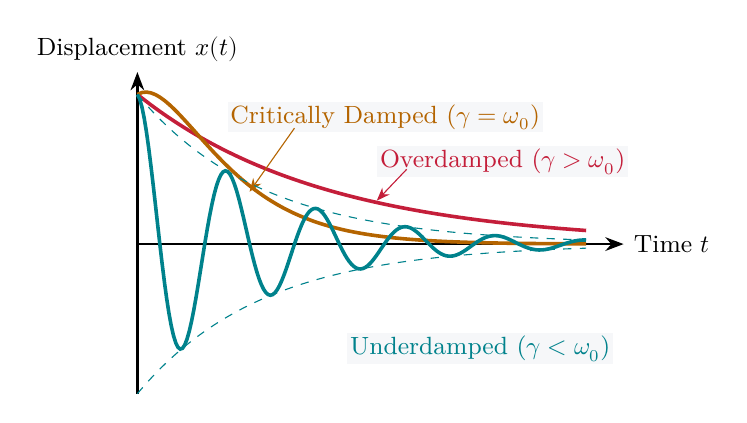
\begin{tikzpicture}[scale=0.95]
  % Axes
  \draw[-Stealth, thick] (0,0) -- (6.5,0) node[right] {\small Time $t$};
  \draw[-Stealth, thick] (0,-2) -- (0,2.3) node[above] {\small Displacement $x(t)$};
  
  % Overdamped curve
  \draw[myred, line width=1.3pt, domain=0:6, samples=100] plot (\x, {2.0*exp(-0.4*\x)});
  \node[myred, fill=mygray, inner sep=1pt, anchor=west] at (3.2, 1.1) {\small Overdamped ($\gamma > \omega_0$)};
  \draw[-Stealth, thin, myred] (3.6, 1.0) -- (3.2, 0.58);
  
  % Critically damped curve
  \draw[myamber, line width=1.3pt, domain=0:6, samples=100] plot (\x, {2.0*(1+1.8*\x)*exp(-1.5*\x)});
  \node[myamber, fill=mygray, inner sep=1pt, anchor=west] at (1.2, 1.7) {\small Critically Damped ($\gamma = \omega_0$)};
  \draw[-Stealth, thin, myamber] (2.1, 1.55) -- (1.5, 0.7);
  
  % Underdamped curve
  \draw[myteal, line width=1.3pt, domain=0:6, samples=200] plot (\x, {2.0*exp(-0.6*\x)*cos(360*\x/1.2)});
  \node[myteal, fill=mygray, inner sep=1pt, anchor=west] at (2.8, -1.4) {\small Underdamped ($\gamma < \omega_0$)};
  
  % Envelope
  \draw[dashed, myteal, thin, domain=0:6, samples=100] plot (\x, {2.0*exp(-0.6*\x)});
  \draw[dashed, myteal, thin, domain=0:6, samples=100] plot (\x, {-2.0*exp(-0.6*\x)});
\end{tikzpicture}
\end{tcolorbox}

% =============================================================================
% QUICK REVISION PAGE
% =============================================================================
\newpage
\begin{center}
  {\large\bfseries\color{myred} Quick Revision --- Module 1}\\[3pt]
  {\small\color{mydark} Mechanics $|$ BS-PH101}
\end{center}
\noindent{\color{myred}\rule{\linewidth}{1.2pt}}
\vspace{4pt}

\begin{tcolorbox}[formulabox, title={\textbf{Key Formulas and Metrics at a Glance}}]
\renewcommand{\arraystretch}{1.35}
\begin{tabularx}{\linewidth}{B{5.0cm} X}
Degrees of Freedom & $f = 3N - k$ \quad ($N$ particles, $k$ constraints) \\[4pt]
Limiting Static Friction & $f_{s,\max} = \mu_s N$ \quad and \quad $\tan\lambda = \mu_s$ \\[4pt]
Potential Energy Relation & $\vec{F} = -\nabla V = -\left(\frac{\partial V}{\partial x}\hat{i} + \frac{\partial V}{\partial y}\hat{j} + \frac{\partial V}{\partial z}\hat{k}\right)$ \\[4pt]
Conservative Force Rule & $\nabla \times \vec{F} = 0 \iff \oint \vec{F} \cdot d\vec{r} = 0$ \\[4pt]
Coriolis Acceleration & $\vec{a}_{\text{cor}} = 2(\vec{\omega} \times \vec{v}')$ \quad (Deflection to right in Northern Hemisphere) \\[4pt]
Underdamped Frequency & $\omega_d = \sqrt{\omega_0^2 - \gamma^2}$ \quad ($\gamma = b/2m$) \\[4pt]
Quality Factor & $Q = \frac{\omega_0}{2\gamma} = \frac{\pi}{\delta} = \omega_0 \tau$ \\[4pt]
Resonance Amplitude Freq. & $\omega_r = \sqrt{\omega_0^2 - 2\gamma^2}$ \\[4pt]
Parallel Axis Theorem & $I = I_{\text{cm}} + M h^2$ \\[4pt]
Perpendicular Axis Theorem & $I_z = I_x + I_y$ \quad (Planar lamina in $xy$-plane) \\[4pt]
\end{tabularx}
\end{tcolorbox}

\begin{tcolorbox}[defbox, title={\textbf{One-Line Definitions}}]
\begin{itemize}[leftmargin=*, itemsep=2pt]
  \item \textbf{Holonomic Constraint:} A constraint expressible as an integrable algebraic equation of position coordinates and time $f(\vec{r}, t) = 0$.
  \item \textbf{Conservative Force:} A force field in which work done along any closed path is zero ($\oint \vec{F} \cdot d\vec{r} = 0$).
  \item \textbf{Coriolis Force:} A velocity-dependent fictitious force acting in a rotating reference frame ($\vec{F}_{\text{cor}} = -2m(\vec{\omega} \times \vec{v}')$).
  \item \textbf{Logarithmic Decrement:} The natural log of ratio of two consecutive amplitudes one period apart ($\delta = \gamma T_d$).
  \item \textbf{Radius of Gyration:} The perpendicular distance from axis of rotation where whole mass can be assumed concentrated ($I = M k^2$).
\end{itemize}
\end{tcolorbox}

\begin{tcolorbox}[exambox, title={\textbf{Frequently Asked / Viva Questions}}]
\begin{enumerate}[topsep=0pt, label=\textbf{Q\arabic*.}, itemsep=5pt]
  \item \Q{State the condition for a force field to be conservative.}
  A force field $\vec{F}$ is conservative if $\nabla \times \vec{F} = 0$ (irrotational) or equivalently work done around any closed loop $\oint \vec{F} \cdot d\vec{r} = 0$.

  \item \Q{Why is Coriolis force called a fictitious force?}
  Because it arises due to the acceleration of the observer's rotating frame of reference, not due to physical interactions between bodies.

  \item \Q{What is the physical significance of negative gradient of potential energy?}
  $\vec{F} = -\nabla V$ indicates force always points in direction of steepest decrease of potential energy towards stable equilibrium.

  \item \Q{Distinguish between holonomic and non-holonomic constraints with examples.}
  Holonomic constraints are integrable algebraic position relations (e.g. rigid body length); non-holonomic involve non-integrable velocity relations or inequalities (e.g. sphere rolling without slipping).

  \item \Q{What is critical damping and state its practical application?}
  Critical damping occurs when $\gamma = \omega_0$. The system returns to equilibrium in shortest time without oscillating. Used in car shock absorbers and deadbeat galvanometers.

  \item \Q{How does amplitude resonance frequency differ from velocity resonance frequency?}
  Amplitude resonance occurs at $\omega_r = \sqrt{\omega_0^2 - 2\gamma^2}$ while velocity resonance occurs exactly at natural frequency $\omega_v = \omega_0$.

  \item \Q{What is Quality Factor ($Q$) of an oscillator?}
  $Q = 2\pi \frac{\text{Energy stored}}{\text{Energy lost per cycle}} = \frac{\omega_0}{2\gamma}$. Higher $Q$ implies lower damping and sharper resonance.

  \item \Q{State Parallel and Perpendicular axes theorems of moment of inertia.}
  Parallel axis: $I = I_{\text{cm}} + Mh^2$. Perpendicular axis: $I_z = I_x + I_y$ for planar laminas.

  \item \Q{Why are track rails laid higher on outer curves?}
  To provide necessary centripetal force via component of normal reaction and eliminate reliance on lateral friction.

  \item \Q{Calculate the moment of inertia of a solid sphere of mass $M$ and radius $R$ about a tangent.}
  By parallel axis theorem, $I_{\text{tangent}} = I_{\text{cm}} + M R^2 = \frac{2}{5}M R^2 + M R^2 = \frac{7}{5}M R^2$.

  \item \Q{What is the total energy of a simple harmonic oscillator of mass $m$ and amplitude $A$?}
  $E = \frac{1}{2} m \omega_0^2 A^2$. Total mechanical energy is constant and continuously converts between kinetic and potential forms.

  \item \Q{Show that Coriolis force does no work on a moving particle.}
  $\vec{F}_{\text{cor}} = -2m(\vec{\omega} \times \vec{v}')$ is always perpendicular to velocity $\vec{v}'$. Power $P = \vec{F}_{\text{cor}} \cdot \vec{v}' = 0 \implies W = 0$.
\end{enumerate}
\end{tcolorbox}

\begin{tcolorbox}[tikzbox, title={Summary Comparison of Damped Motion Regimes}]
\centering
\begin{tabularx}{\linewidth}{|B{3.0cm}|Y|Y|Y|}
\hline
\textbf{Parameter} & \textbf{Overdamped ($\gamma > \omega_0$)} & \textbf{Critically Damped ($\gamma = \omega_0$)} & \textbf{Underdamped ($\gamma < \omega_0$)} \\
\hline
\textbf{Roots of Char. Eq.} & Real and distinct. & Real and equal ($r = -\gamma$). & Complex conjugate ($-\gamma \pm i\omega_d$). \\
\hline
\textbf{Motion Nature} & Non-oscillatory, slow return. & Non-oscillatory, fastest return. & Oscillatory with decaying amplitude. \\
\hline
\textbf{Frequency} & No frequency of oscillation. & No frequency of oscillation. & $\omega_d = \sqrt{\omega_0^2 - \gamma^2}$. \\
\hline
\textbf{Practical Use} & Heavy door closers. & Galvanometers, vehicle suspension. & Tuning circuits, musical strings. \\
\hline
\end{tabularx}
\end{tcolorbox}


% -- Module 2 -----------------------------------------------------------------
\modulestart{2}{Interference vs. Diffraction and Classification}

\section{Interference vs. Diffraction and Classification}

\subsection{Distinction Between Interference and Diffraction}

\begin{tcolorbox}[defbox, title={\textbf{Definition: Interference and Diffraction}}]
\begin{itemize}[leftmargin=*, itemsep=2pt]
  \item \textbf{Interference:} Modification in intensity resulting from the superposition of two or more coherent light waves originating from distinct coherent sources.
  \item \textbf{Diffraction:} The bending of light waves around the sharp edges of an obstacle or aperture and their subsequent superposition within the geometrical shadow region.
\end{itemize}
\end{tcolorbox}

\textbf{Comprehensive Comparison:}\par\vspace{6pt}\noindent
\begin{tabularx}{\linewidth}{|B{3.2cm}|Y|Y|}
\hline
\textbf{Property} & \textbf{Interference} & \textbf{Diffraction} \\
\hline
\textbf{Wave Origin} & Superposition of waves from two distinct coherent sources. & Superposition of secondary wavelets originating from different points of the \textit{same} wavefront. \\
\hline
\textbf{Fringe Width} & Fringes are usually of equal width ($\beta = \lambda D / d$). & Fringes are never of equal width (central max is twice as wide as secondary max). \\
\hline
\textbf{Intensity} & All bright fringes have equal intensity ($I_{\max} = 4 I_0$). & Intensity decreases rapidly with increasing order of secondary maxima. \\
\hline
\textbf{Darkness} & Minima are completely dark ($I_{\min} = 0$). & Minima are generally not completely dark. \\
\hline
\end{tabularx}

\subsection{Fraunhofer vs. Fresnel Diffraction}

\begin{tabularx}{\linewidth}{|B{3.2cm}|Y|Y|}
\hline
\textbf{Feature} & \textbf{Fresnel Diffraction} & \textbf{Fraunhofer Diffraction} \\
\hline
\textbf{Distance} & Source and screen are at finite distances from aperture. & Source and screen are at effectively infinite distances. \\
\hline
\textbf{Wavefront} & Incident wavefront is spherical or cylindrical. & Incident wavefront is plane (parallel rays). \\
\hline
\textbf{Lenses} & No lenses required to focus pattern. & Convex lenses required before and after aperture. \\
\hline
\textbf{Analysis} & Analyzed using Fresnel half-period zones. & Analyzed using simple wave phase summation. \\
\hline
\end{tabularx}

% =============================================================================
% SECTION 2: FRAUNHOFER DIFFRACTION
% =============================================================================
\section{Fraunhofer Diffraction at Single, Double, and Multiple Slits}

\subsection{Single Slit Diffraction}

Consider a plane wavefront of wavelength $\lambda$ incident normally on a slit of width $e$.

\begin{tcolorbox}[formulabox, title={\textbf{Single Slit Intensity Formula}}]
The resultant intensity on a screen at diffraction angle $\theta$ is:
\begin{equation}
I(\theta) = I_0 \left(\frac{\sin \beta}{\beta}\right)^2 \quad \text{where } \beta = \frac{\pi e \sin \theta}{\lambda}
\end{equation}
\end{tcolorbox}

\textbf{Key Conditions:}\par\noindent
\begin{itemize}[leftmargin=*, itemsep=3pt]
  \item \textbf{Central Maximum:} At $\theta = 0 \implies \beta = 0$, $\lim_{\beta\to 0} \frac{\sin\beta}{\beta} = 1 \implies I = I_0$.
  \item \textbf{Minima Condition:} $\sin \beta = 0$ (for $\beta \neq 0$) $\implies \beta = m \pi \implies e \sin \theta = m \lambda \quad (m = \pm 1, \pm 2, \pm 3, \ldots)$.
  \item \textbf{Secondary Maxima:} Occur near $\beta = \pm 1.43 \pi, \pm 2.46 \pi, \dots$ with intensity ratios:
  \begin{equation}
  I_0 : I_1 : I_2 = 1 : \frac{1}{22} : \frac{1}{61} = 1 : 0.045 : 0.016
  \end{equation}
  \item \textbf{Width of Central Maximum:} $\Delta \theta = \frac{2 \lambda}{e} \implies \text{Linear Width } W = \frac{2 \lambda f}{e}$ (where $f$ is lens focal length).
\end{itemize}

\subsection{Double Slit Diffraction}

For two parallel slits, each of width $e$ and separated by opaque spacing $d$ (grating element $= e + d$):

\begin{tcolorbox}[formulabox, title={\textbf{Double Slit Intensity Formula}}]
\begin{equation}
I(\theta) = 4 I_0 \left(\frac{\sin \beta}{\beta}\right)^2 \cos^2 \alpha \quad \text{where } \beta = \frac{\pi e \sin \theta}{\lambda}, \;\; \alpha = \frac{\pi (e+d) \sin \theta}{\lambda}
\end{equation}
It is the product of single-slit diffraction factor $\left(\frac{\sin\beta}{\beta}\right)^2$ and interference factor $\cos^2\alpha$.
\end{tcolorbox}

\textbf{Missing Orders (Absent Spectra):} Occurs when an interference maximum coincides with a diffraction minimum:
\begin{equation}
(e+d)\sin\theta = n \lambda \quad \text{and} \quad e\sin\theta = m \lambda \implies \frac{e+d}{e} = \frac{n}{m}
\end{equation}
If $e = d$, then $\frac{n}{m} = 2 \implies n = 2m$, so $2^{\text{nd}}, 4^{\text{th}}, 6^{\text{th}}$ interference orders disappear.

\subsection{Diffraction Grating and Resolving Power}

A plane transmission diffraction grating consists of $N$ parallel, equally spaced slits with grating element $(e+d)$.

\begin{tcolorbox}[formulabox, title={\textbf{Grating Equations and Resolving Power}}]
\begin{itemize}[leftmargin=*, itemsep=3pt]
  \item \textbf{Principal Maxima Condition:}
  \begin{equation}
  (e+d)\sin\theta = m \lambda \quad (m = 0, 1, 2, \ldots)
  \end{equation}
  \item \textbf{Dispersive Power ($D$):} Rate of change of diffraction angle with wavelength:
  \begin{equation}
  D = \frac{d\theta}{d\lambda} = \frac{m}{(e+d)\cos\theta}
  \end{equation}
  \item \textbf{Resolving Power ($R$):} Capacity to separate two spectral lines of wavelength $\lambda$ and $\lambda + d\lambda$:
  \begin{equation}
  R = \frac{\lambda}{d\lambda} = m N \quad (N = \text{total illuminated rulings})
  \end{equation}
\end{itemize}
\end{tcolorbox}

\begin{tcolorbox}[examplebox, title={\textbf{Solved Problem 1: Grating Spectral Lines and Maximum Order}}]
\textbf{Problem:} A grating has $5000\text{ lines/cm}$. Light of wavelength $\lambda = 6000\text{ \AA}$ is incident normally. Find: (a) Grating element $(e+d)$, (b) Highest observable order.

\textbf{Solution:}\par\noindent
\begin{enumerate}[leftmargin=*, itemsep=2pt]
  \item Grating element $(e+d) = \frac{1\text{ cm}}{5000} = 2 \times 10^{-4}\text{ cm} = 2 \times 10^{-6}\text{ m}$.
  \item Maximum angle $\theta_{\max} = 90^\circ \implies \sin 90^\circ = 1$.
  \item Substitute in grating equation $(e+d)\sin 90^\circ = m_{\max} \lambda$:
   \begin{equation}
   m_{\max} = \frac{(e+d)}{\lambda} = \frac{2 \times 10^{-6}\text{ m}}{600 \times 10^{-9}\text{ m}} = 3.33 \implies \mathbf{m_{\max} = 3}
   \end{equation}
\end{enumerate}
Hence, maximum $3^{\text{rd}}$ order spectrum can be observed.
\end{tcolorbox}

\begin{tcolorbox}[examplebox, title={\textbf{Solved Problem 2: Single Slit Central Width}}]
\textbf{Problem:} Light of wavelength $\lambda = 5890\text{ \AA}$ is incident normally on a slit of width $0.1\text{ mm}$. A convex lens of focal length $f = 1.0\text{ m}$ is placed behind the slit. Calculate linear width of central maximum.

\textbf{Solution:}\par\noindent
Linear width of central maximum $W = \frac{2 \lambda f}{e}$.
$W = \frac{2 \times 5890 \times 10^{-10}\text{ m} \times 1.0\text{ m}}{0.1 \times 10^{-3}\text{ m}} = 11.78 \times 10^{-3}\text{ m} = \mathbf{11.78\text{ mm}}$.
\end{tcolorbox}

% =============================================================================
% SECTION 3: POLARISATION OF LIGHT
% =============================================================================
\section{Polarisation of Light}

\subsection{Brewster's Law and Double Refraction}

\begin{tcolorbox}[defbox, title={\textbf{Brewster's Law}}]
When unpolarised light is incident at a specific angle $i_p$ (polarising angle) on a dielectric interface, the reflected light is $100\%$ plane polarised with electric vector perpendicular to plane of incidence.
\begin{equation}
\mu = \tan i_p \quad \text{and} \quad i_p + r = 90^\circ
\end{equation}
\end{tcolorbox}

\begin{tcolorbox}[tikzbox, title={Polarisation by Reflection (Brewster's Law)}]
\centering
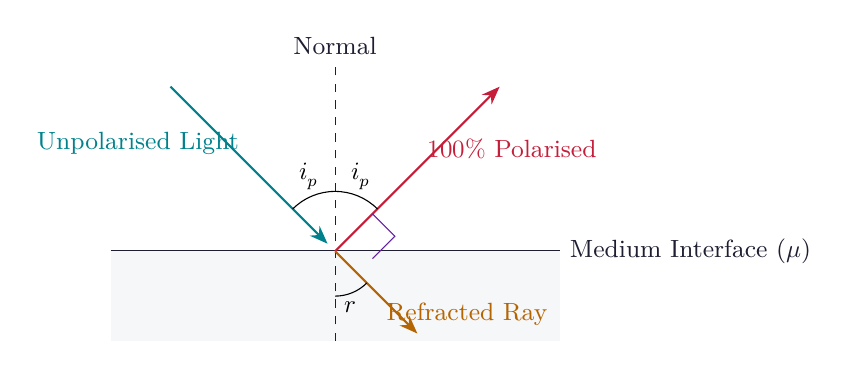
\begin{tikzpicture}[scale=0.95]
  % Boundary
  \draw[thick, mydark] (-3,0) -- (3,0) node[right] {\small Medium Interface ($\mu$)};
  \fill[mygray] (-3,-1.2) rectangle (3,0);
  
  % Normal
  \draw[dashed, mydark] (0,-1.2) -- (0,2.5) node[above] {\small Normal};
  
  % Rays
  \draw[thick, myteal, -Stealth] (-2.2,2.2) -- (-0.1,0.1) node[midway, above left] {\small Unpolarised Light};
  \draw[thick, myred, -Stealth] (0,0) -- (2.2,2.2) node[midway, above right] {\small $100\%$ Polarised};
  \draw[thick, myamber, -Stealth] (0,0) -- (1.1,-1.1) node[midway, below right] {\small Refracted Ray};
  
  % Angles
  \draw[thin] (0,0.8) arc (90:135:0.8);
  \node at (-0.35,1.0) {\small $i_p$};
  \draw[thin] (0,0.8) arc (90:45:0.8);
  \node at (0.35,1.0) {\small $i_p$};
  \draw[thin] (0,-0.6) arc (270:315:0.6);
  \node at (0.2,-0.75) {\small $r$};
  
  % 90 deg marker between reflected and refracted
  \draw[thin, mypurple] (0.5,0.5) -- (0.8,0.2) -- (0.5,-0.1);
\end{tikzpicture}
\end{tcolorbox}

\textbf{Double Refraction (Birefringence):} When unpolarised light enters an anisotropic crystal (e.g. Calcite, Quartz), it splits into two plane polarised rays travelling at different speeds:
\begin{itemize}[leftmargin=*, itemsep=2pt]
  \item \textbf{Ordinary Ray ($O$-ray):} Obeys Snell's law; travels with equal velocity in all directions ($v_o = c/\mu_o$).
  \item \textbf{Extraordinary Ray ($E$-ray):} Violates Snell's law; velocity depends on direction of propagation ($v_e$).
\end{itemize}

\subsection{Retardation Plates: Quarter-Wave and Half-Wave Plates}

\begin{tcolorbox}[formulabox, title={\textbf{Retardation Plate Thickness Equations}}]
For a crystal plate cut parallel to optic axis of thickness $t$:
\begin{itemize}[leftmargin=*, itemsep=3pt]
  \item \textbf{Quarter-Wave Plate (QWP):} Introduces phase difference $\Delta \phi = \pi/2$ or path difference $\Delta x = \lambda/4$:
  \begin{equation}
  t = \frac{\lambda}{4 |\mu_o - \mu_e|}
  \end{equation}
  \item \textbf{Half-Wave Plate (HWP):} Introduces phase difference $\Delta \phi = \pi$ or path difference $\Delta x = \lambda/2$:
  \begin{equation}
  t = \frac{\lambda}{2 |\mu_o - \mu_e|}
  \end{equation}
\end{itemize}
\end{tcolorbox}

\subsection{Optical Activity and Laurent's Half-Shade Polarimeter}

Optically active substances rotate the plane of polarization of linearly polarized light.
The angle of rotation $\theta$ is given by Biot's law: $\theta = S \cdot L \cdot c$.
\begin{equation}
\text{Specific Rotation } [S]_\lambda^T = \frac{\theta}{L \cdot c} \quad \left(\text{in } \frac{\text{deg}}{\text{dm} \cdot \text{g/cm}^3}\right)
\end{equation}
where $\theta = \text{rotation angle (deg)}$, $L = \text{path length in decimeters (dm)}$, $c = \text{concentration in g/cm}^3$.

\textbf{Laurent's Half-Shade Polarimeter:} Uses a half-shade plate (half quartz, half glass) to divide the field of view into two halves, enabling precise setting of equal brightness.

\begin{tcolorbox}[examplebox, title={\textbf{Solved Problem 3: Quarter-Wave Plate Thickness}}]
\textbf{Problem:} Calculate the minimum thickness of a quarter-wave plate of Calcite for sodium light of wavelength $\lambda = 5893\text{ \AA}$. Given $\mu_o = 1.6583$ and $\mu_e = 1.4864$.

\textbf{Solution:}\par\noindent
\begin{enumerate}[leftmargin=*, itemsep=2pt]
  \item Calcite is a negative crystal ($\mu_o > \mu_e$), so $|\mu_o - \mu_e| = 1.6583 - 1.4864 = 0.1719$.
  \item Formula: $t = \frac{\lambda}{4(\mu_o - \mu_e)}$.
  \item Substitute: $t = \frac{5893 \times 10^{-10}\text{ m}}{4 \times 0.1719} = \frac{5893 \times 10^{-10}}{0.6876} = 8570 \times 10^{-10}\text{ m} = \mathbf{0.857\text{ \mu m}}$.
\end{enumerate}
\end{tcolorbox}

% =============================================================================
% SECTION 4: LASERS
% =============================================================================
\section{Lasers (Light Amplification by Stimulated Emission of Radiation)}

\subsection{Principles of Laser Action: Einstein's Coefficients}

Interaction of radiation with matter involves three fundamental processes:

\begin{tcolorbox}[formulabox, title={\textbf{Three Radiation Processes and Einstein's Relations}}]
\begin{enumerate}[leftmargin=*, itemsep=3pt]
  \item \textbf{Stimulated Absorption:} Atom absorbs photon: Rate $R_{12} = B_{12} N_1 u(\nu)$.
  \item \textbf{Spontaneous Emission:} Atom decays naturally: Rate $R_{21,\text{sp}} = A_{21} N_2$.
  \item \textbf{Stimulated Emission:} Incident photon induces decay: Rate $R_{21,\text{st}} = B_{21} N_2 u(\nu)$.
\end{enumerate}
At thermal equilibrium, $R_{12} = R_{21,\text{sp}} + R_{21,\text{st}}$. Equating with Planck's law yields Einstein's relations:
\begin{equation}
B_{12} = B_{21} \quad \text{and} \quad \frac{A_{21}}{B_{21}} = \frac{8\pi h \nu^3}{c^3}
\end{equation}
\end{tcolorbox}

\subsection{Population Inversion and Pumping}

Under normal thermal equilibrium (Boltzmann distribution $N_2 = N_1 e^{-h\nu/kT}$), $N_1 \gg N_2$.

\begin{tcolorbox}[defbox, title={\textbf{Definition: Population Inversion and Pumping}}]
\begin{itemize}[leftmargin=*, itemsep=2pt]
  \item \textbf{Population Inversion:} The non-equilibrium state in which higher energy level population exceeds lower energy level ($N_2 > N_1$). Necessary condition for optical amplification.
  \item \textbf{Pumping:} The external process of supplying energy to raise atoms to higher excited levels to achieve population inversion (e.g. Optical pumping, Electrical discharge, Direct electron excitation).
  \item \textbf{Metastable State:} An excited state with a long lifetime ($\sim 10^{-3}\text{ s}$ compared to normal $10^{-8}\text{ s}$), allowing accumulation of atoms for population inversion.
\end{itemize}
\end{tcolorbox}

\subsection{He-Ne Laser (Gas Laser)}

\begin{tcolorbox}[tikzbox, title={He-Ne Laser Energy Level Diagram}]
\centering
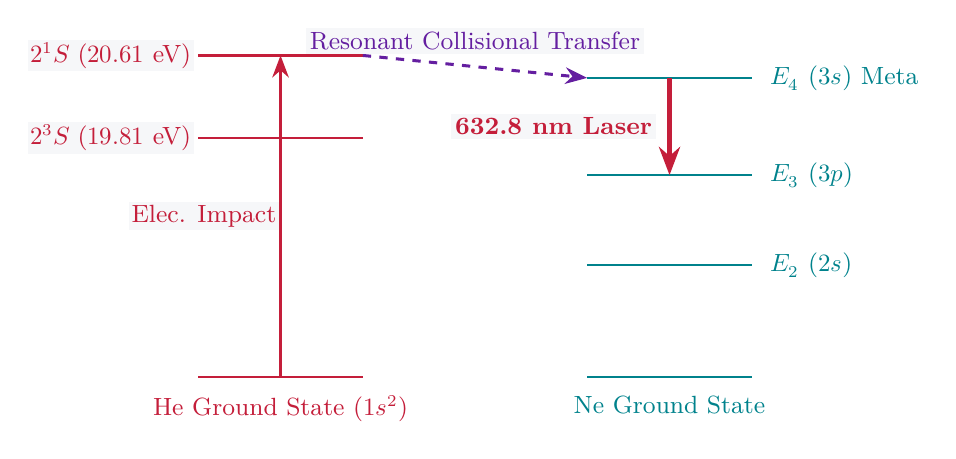
\begin{tikzpicture}[scale=0.95]
  % He Levels (Left)
  \draw[thick, myred] (0.6,0) -- (2.8,0) node[midway, below=3pt] {\small He Ground State ($1s^2$)};
  \draw[thick, myred] (0.6,3.2) -- (2.8,3.2);
  \node[myred, fill=mygray, inner sep=1pt, anchor=east] at (0.55, 3.2) {\small $2^3S$ ($19.81\text{ eV}$)};
  
  \draw[thick, myred] (0.6,4.3) -- (2.8,4.3);
  \node[myred, fill=mygray, inner sep=1pt, anchor=east] at (0.55, 4.3) {\small $2^1S$ ($20.61\text{ eV}$)};
  
  % Ne Levels (Right)
  \draw[thick, myteal] (5.8,0) -- (8.0,0) node[midway, below=3pt] {\small Ne Ground State};
  \draw[thick, myteal] (5.8,1.5) -- (8.0,1.5) node[right=3pt] {\small $E_2$ ($2s$)};
  \draw[thick, myteal] (5.8,2.7) -- (8.0,2.7) node[right=3pt] {\small $E_3$ ($3p$)};
  \draw[thick, myteal] (5.8,4.0) -- (8.0,4.0) node[right=3pt] {\small $E_4$ ($3s$) Meta};
  
  % Excitation & Transfer
  \draw[-Stealth, redarrow, line width=1.1pt] (1.7,0) -- (1.7,4.3) node[midway, fill=mygray, inner sep=1pt, anchor=east] {\small Elec. Impact};
  \draw[-Stealth, dashed, line width=1.1pt, mypurple] (2.8,4.3) -- (5.8,4.0) node[midway, above=4pt, fill=mygray, inner sep=1.5pt] {\small Resonant Collisional Transfer};
  
  % Laser Transition (Arrow on right, text on left of arrow)
  \draw[-Stealth, line width=1.6pt, myred] (6.9,4.0) -- (6.9,2.7) node[midway, left=4pt, fill=mygray, inner sep=1.5pt] {\small\textbf{632.8 nm Laser}};
\end{tikzpicture}
\end{tcolorbox}

\textbf{Working Mechanism of He-Ne Laser:}
\begin{enumerate}[leftmargin=*, itemsep=2pt]
  \item Electric discharge accelerates electrons which excite He atoms to metastable $2^1S$ ($20.61\text{ eV}$) state.
  \item He atoms transfer energy to Ne atoms via resonant inelastic collisions, populating Ne's $3s$ ($E_4$) level.
  \item Stimulated emission from $3s \to 2p$ ($E_4 \to E_3$) produces red laser light at $\lambda = 632.8\text{ nm}$.
\end{enumerate}

% =============================================================================
% QUICK REVISION PAGE
% =============================================================================
\newpage
\begin{center}
  {\large\bfseries\color{myred} Quick Revision --- Module 2}\\[3pt]
  {\small\color{mydark} Optics $|$ BS-PH101}
\end{center}
\noindent{\color{myred}\rule{\linewidth}{1.2pt}}
\vspace{4pt}

\begin{tcolorbox}[formulabox, title={\textbf{Key Formulas and Metrics at a Glance}}]
\renewcommand{\arraystretch}{1.35}
\begin{tabularx}{\linewidth}{B{5.0cm} X}
Single Slit Minima & $e \sin\theta = m \lambda \quad (m = \pm 1, \pm 2, \ldots)$ \\[4pt]
Single Slit Central Width & $\Delta \theta = \frac{2\lambda}{e} \implies \text{Linear Width } W = \frac{2\lambda f}{e}$ \\[4pt]
Double Slit Missing Orders & $\frac{e+d}{e} = \frac{n}{m} \quad (n = \text{interf. order}, m = \text{diff. order})$ \\[4pt]
Grating Equation & $(e+d)\sin\theta = m \lambda$ \\[4pt]
Grating Dispersive Power & $D = \frac{d\theta}{d\lambda} = \frac{m}{(e+d)\cos\theta}$ \\[4pt]
Grating Resolving Power & $R = \frac{\lambda}{d\lambda} = m N$ \\[4pt]
Brewster's Law & $\mu = \tan i_p \quad \text{and} \quad i_p + r = 90^\circ$ \\[4pt]
Quarter-Wave Plate (QWP) & $t = \frac{\lambda}{4 |\mu_o - \mu_e|}$ \\[4pt]
Half-Wave Plate (HWP) & $t = \frac{\lambda}{2 |\mu_o - \mu_e|}$ \\[4pt]
Specific Rotation & $[S]_\lambda^T = \frac{\theta}{L \cdot c} \quad (\text{deg} \cdot \text{dm}^{-1} \cdot (\text{g/cm}^3)^{-1})$ \\[4pt]
Einstein Coefficients Relation & $\frac{A_{21}}{B_{21}} = \frac{8\pi h \nu^3}{c^3} \quad \text{and} \quad B_{12} = B_{21}$ \\[4pt]
\end{tabularx}
\end{tcolorbox}

\begin{tcolorbox}[defbox, title={\textbf{One-Line Definitions}}]
\begin{itemize}[leftmargin=*, itemsep=2pt]
  \item \textbf{Diffraction Grating:} An optical component with a periodic structure of $N$ slits that diffracts light into several beams.
  \item \textbf{Brewster Angle ($i_p$):} Angle of incidence at which light with a particular polarization is perfectly transmitted without reflection.
  \item \textbf{Birefringence:} The optical property of a material having a refractive index that depends on the polarization and propagation direction of light.
  \item \textbf{Population Inversion:} State in which a system exists with more members in an excited state than in lower energy states ($N_2 > N_1$).
  \item \textbf{Metastable State:} An excited atomic state with a long lifetime ($\sim 10^{-3}\text{ s}$), essential for building up population inversion.
\end{itemize}
\end{tcolorbox}

\begin{tcolorbox}[exambox, title={\textbf{Frequently Asked / Viva Questions}}]
\begin{enumerate}[topsep=0pt, label=\textbf{Q\arabic*.}, itemsep=5pt]
  \item \Q{What is the basic difference between interference and diffraction?}
  Interference results from superposition of waves from two distinct coherent sources; diffraction results from superposition of wavelets from different parts of the same wavefront.

  \item \Q{Why is central maximum in single-slit diffraction twice as wide as secondary maxima?}
  Because central maximum extends between first minima on either side ($\sin\theta = \pm \lambda/e$), spanning angular width $2\lambda/e$, whereas secondary maxima span width $\lambda/e$.

  \item \Q{What is meant by missing orders in double slit diffraction?}
  Missing orders occur when an interference maximum coincides with a diffraction minimum at the same angle $\theta$, making that order absent ($\frac{e+d}{e} = \frac{n}{m}$).

  \item \Q{State Rayleigh's criterion for spectral resolution.}
  Two spectral lines are just resolved when the central principal maximum of one falls on the first minimum of the other.

  \item \Q{How does resolving power of a grating differ from dispersive power?}
  Dispersive power ($d\theta/d\lambda$) measures angular separation between lines; resolving power ($\lambda/d\lambda = mN$) measures ability to distinguish two close wavelengths.

  \item \Q{State Brewster's law and show reflected and refracted rays are perpendicular.}
  $\mu = \tan i_p$. Since $\frac{\sin i_p}{\sin r} = \tan i_p = \frac{\sin i_p}{\cos i_p} \implies \sin r = \cos i_p = \sin(90^\circ - i_p) \implies i_p + r = 90^\circ$.

  \item \Q{What are $O$-ray and $E$-ray in a birefringent crystal?}
  $O$-ray (Ordinary) obeys Snell's law with constant speed $v_o$; $E$-ray (Extraordinary) violates Snell's law with directional speed $v_e$.

  \item \Q{Distinguish between positive and negative uniaxial crystals.}
  In positive crystals ($\mu_e > \mu_o$, e.g. Quartz), $v_o > v_e$; in negative crystals ($\mu_o > \mu_e$, e.g. Calcite), $v_e > v_o$.

  \item \Q{Explain the function of a Quarter-Wave Plate (QWP).}
  A QWP introduces a path difference of $\lambda/4$ ($\pi/2$ phase shift) between $O$-ray and $E$-ray, converting linearly polarized light to circularly or elliptically polarized light.

  \item \Q{What is population inversion and why is it necessary for laser action?}
  Population inversion ($N_2 > N_1$) ensures that rate of stimulated emission exceeds rate of stimulated absorption, producing net optical amplification.

  \item \Q{Why is Helium gas added to Neon gas in a He-Ne laser?}
  He atoms are excited by electron impact to metastable states ($2^1S, 2^3S$) and efficiently transfer energy to Ne atoms via resonant collisions, achieving population inversion in Ne.

  \item \Q{Derive relation between Einstein $A$ and $B$ coefficients.}
  Equating thermal equilibrium rate $B_{12} N_1 u(\nu) = A_{21} N_2 + B_{21} N_2 u(\nu)$ with Boltzmann distribution $N_2/N_1 = e^{-h\nu/kT}$ and Planck's radiation law gives $B_{12} = B_{21}$ and $A_{21}/B_{21} = 8\pi h\nu^3/c^3$.
\end{enumerate}
\end{tcolorbox}

\begin{tcolorbox}[tikzbox, title={Summary Comparison of Laser Processes}]
\centering
\begin{tabularx}{\linewidth}{|B{3.2cm}|Y|Y|Y|}
\hline
\textbf{Process} & \textbf{Incident Condition} & \textbf{Transition} & \textbf{Output Properties} \\
\hline
\textbf{Absorption} & Photon ($h\nu = E_2 - E_1$) & Lower $E_1 \to$ Higher $E_2$ & Atom reaches excited state. \\
\hline
\textbf{Spontaneous Emission} & Natural decay (lifetime $\sim 10^{-8}\text{s}$) & Higher $E_2 \to$ Lower $E_1$ & Incoherent, random phase/direction. \\
\hline
\textbf{Stimulated Emission} & Triggering photon ($h\nu$) & Higher $E_2 \to$ Lower $E_1$ & Coherent, identical phase, direction, and wavelength. \\
\hline
\end{tabularx}
\end{tcolorbox}


% -- Module 3 -----------------------------------------------------------------
\modulestart{3}{Maxwell's Equations and Electromagnetic Waves}

\section{Maxwell's Equations and Electromagnetic Waves}

\subsection{Maxwell's Four Fundamental Equations}

Maxwell unified electricity and magnetism into four differential and integral equations governing electromagnetic phenomena.

\begin{tcolorbox}[formulabox, title={\textbf{Maxwell's Equations in Differential and Integral Forms}}]
\begin{enumerate}[leftmargin=*, itemsep=4pt]
  \item \textbf{Gauss's Law for Electrostatics:} Net electric flux through a closed surface equals charge enclosed:
  \begin{equation}
  \nabla \cdot \vec{D} = \rho \iff \oint_S \vec{D} \cdot d\vec{A} = Q_{\text{enclosed}} \quad (\vec{D} = \epsilon_0 \vec{E} + \vec{P})
  \end{equation}
  \item \textbf{Gauss's Law for Magnetostatics:} Magnetic monopoles do not exist (magnetic flux lines are continuous loops):
  \begin{equation}
  \nabla \cdot \vec{B} = 0 \iff \oint_S \vec{B} \cdot d\vec{A} = 0
  \end{equation}
  \item \textbf{Faraday's Law of Electromagnetic Induction:} Time-varying magnetic field produces an electric field:
  \begin{equation}
  \nabla \times \vec{E} = -\frac{\partial \vec{B}}{\partial t} \iff \oint_C \vec{E} \cdot d\vec{r} = -\frac{\partial}{\partial t}\int_S \vec{B} \cdot d\vec{A}
  \end{equation}
  \item \textbf{Ampere-Maxwell Law:} Magnetic fields are generated by electric currents and time-varying electric fields:
  \begin{equation}
  \nabla \times \vec{H} = \vec{J} + \frac{\partial \vec{D}}{\partial t} \iff \oint_C \vec{H} \cdot d\vec{r} = \int_S \left(\vec{J} + \frac{\partial \vec{D}}{\partial t}\right) \cdot d\vec{A}
  \end{equation}
\end{enumerate}
\end{tcolorbox}

\subsection{Displacement Current and Wave Equation in Free Space}

Maxwell modified Ampere's law ($\nabla \times \vec{H} = \vec{J}$) by taking the divergence of both sides. Since $\nabla \cdot (\nabla \times \vec{H}) = 0$, it required $\nabla \cdot \vec{J} = 0$, which violates the charge continuity equation $\nabla \cdot \vec{J} + \frac{\partial \rho}{\partial t} = 0$ for time-varying fields.

Substituting $\rho = \nabla \cdot \vec{D}$ into continuity equation:
\begin{equation}
\nabla \cdot \vec{J} + \frac{\partial}{\partial t}(\nabla \cdot \vec{D}) = 0 \implies \nabla \cdot \left( \vec{J} + \frac{\partial \vec{D}}{\partial t} \right) = 0
\end{equation}
Thus, Maxwell introduced the \textbf{Displacement Current Density} $\vec{J}_d = \frac{\partial \vec{D}}{\partial t} = \epsilon_0 \frac{\partial \vec{E}}{\partial t}$.

\begin{tcolorbox}[formulabox, title={\textbf{Electromagnetic Wave Equation and Speed of Light}}]
In free space ($\rho = 0, \vec{J} = 0, \mu = \mu_0, \epsilon = \epsilon_0$), taking curl of Faraday's law yields:
\begin{equation}
\nabla \times (\nabla \times \vec{E}) = -\frac{\partial}{\partial t}(\nabla \times \vec{B}) \implies \nabla(\nabla \cdot \vec{E}) - \nabla^2 \vec{E} = -\mu_0 \epsilon_0 \frac{\partial^2 \vec{E}}{\partial t^2}
\end{equation}
Since $\nabla \cdot \vec{E} = 0$, this simplifies to the standard 3D wave equation:
\begin{equation}
\nabla^2 \vec{E} = \mu_0 \epsilon_0 \frac{\partial^2 \vec{E}}{\partial t^2} \quad \text{and} \quad \nabla^2 \vec{B} = \mu_0 \epsilon_0 \frac{\partial^2 \vec{B}}{\partial t^2}
\end{equation}
Comparing with $\nabla^2 \psi = \frac{1}{v^2}\frac{\partial^2\psi}{\partial t^2}$, the wave velocity in vacuum is:
\begin{equation}
c = \frac{1}{\sqrt{\mu_0 \epsilon_0}} = \frac{1}{\sqrt{(4\pi \times 10^{-7}) (8.854 \times 10^{-12})}} = 2.998 \times 10^8 \text{ m/s}
\end{equation}
\end{tcolorbox}

\subsection{Poynting Vector and Energy Flow}

\begin{tcolorbox}[defbox, title={\textbf{Definition: Poynting Vector}}]
The \textbf{Poynting Vector ($\vec{S}$)} represents the directional energy flux density (rate of energy transfer per unit area) of an electromagnetic field:
\begin{equation}
\vec{S} = \vec{E} \times \vec{H} \quad \left(\text{in } \frac{\text{W}}{\text{m}^2}\right)
\end{equation}
The time-averaged Poynting vector intensity for a plane wave is $I = \langle S \rangle = \frac{1}{2} c \epsilon_0 E_0^2$.
\end{tcolorbox}

\begin{tcolorbox}[examplebox, title={\textbf{Solved Problem 1: Displacement Current in a Capacitor}}]
\textbf{Problem:} A parallel-plate capacitor with circular plates of radius $R = 0.1\text{ m}$ is being charged by a current $I = 2.0\text{ A}$. Calculate: (a) Displacement current $I_d$, (b) Rate of change of electric field $dE/dt$.

\textbf{Solution:}\par\noindent
\begin{enumerate}[leftmargin=*, itemsep=2pt]
  \item Total displacement current between plates equals conduction current in wires: $\mathbf{I_d = 2.0\text{ A}}$.
  \item Plate area $A = \pi R^2 = \pi (0.1)^2 = 0.0314\text{ m}^2$.
  \item $I_d = \epsilon_0 A \frac{dE}{dt} \implies \frac{dE}{dt} = \frac{I_d}{\epsilon_0 A}$:
   \begin{equation}
   \frac{dE}{dt} = \frac{2.0}{(8.854 \times 10^{-12}) \times 0.0314} = \mathbf{7.19 \times 10^{11}\text{ V/(m}\cdot\text{s)}}
   \end{equation}
\end{enumerate}
\end{tcolorbox}

% =============================================================================
% SECTION 2: DIELECTRIC PROPERTIES OF MATERIALS
% =============================================================================
\section{Dielectric Properties of Materials}

\subsection{Dielectric Vectors: Polarisation, Susceptibility, Permittivity}

Dielectrics are electrical insulators that can be polarized by an applied electric field.

\begin{tcolorbox}[formulabox, title={\textbf{Fundamental Dielectric Relations}}]
\begin{itemize}[leftmargin=*, itemsep=3pt]
  \item \textbf{Electric Dipole Moment ($\vec{p}$):} $\vec{p} = q \vec{d}$ (directed from $-q$ to $+q$).
  \item \textbf{Polarisation Vector ($\vec{P}$):} Dipole moment per unit volume: $\vec{P} = N \vec{p}$.
  \item \textbf{Electric Displacement ($\vec{D}$):}
  \begin{equation}
  \vec{D} = \epsilon_0 \vec{E} + \vec{P} = \epsilon_0 \epsilon_r \vec{E}
  \end{equation}
  \item \textbf{Electric Susceptibility ($\chi_e$):} $\vec{P} = \epsilon_0 \chi_e \vec{E} \implies \epsilon_r = 1 + \chi_e$.
\end{itemize}
\end{tcolorbox}

\textbf{Microscopic Polarisation Mechanisms:}\par\vspace{6pt}\noindent
\begin{tabularx}{\linewidth}{|B{3.2cm}|Y|Y|}
\hline
\textbf{Mechanism} & \textbf{Origin / Description} & \textbf{Temperature Dependence} \\
\hline
\textbf{Electronic ($\alpha_e$)} & Displacement of electron cloud relative to nucleus in an atom. & Independent of temperature ($T$). \\
\hline
\textbf{Ionic ($\alpha_i$)} & Relative displacement of positive and negative ions in a crystal lattice. & Independent of temperature ($T$). \\
\hline
\textbf{Orientational ($\alpha_o$)} & Realignment of permanent molecular dipoles along external field. & Strongly temperature dependent ($\alpha_o \propto 1/T$). \\
\hline
\textbf{Space-Charge ($\alpha_s$)} & Accumulation of free charge carriers at interfaces/grain boundaries. & Dependent on temperature and frequency. \\
\hline
\end{tabularx}

\subsection{Clausius-Mossotti Equation}

Consider a solid dielectric where local field acting on an atom is the \textbf{Lorentz Field}:
\begin{equation}
E_{\text{local}} = E + \frac{P}{3\epsilon_0}
\end{equation}
The induced dipole moment per atom is $p = \alpha E_{\text{local}}$, so total polarisation for $N$ atoms per unit volume is:
\begin{equation}
P = N p = N \alpha E_{\text{local}} = N \alpha \left( E + \frac{P}{3\epsilon_0} \right)
\end{equation}

\begin{tcolorbox}[formulabox, title={\textbf{Clausius-Mossotti Relation Derivation}}]
Solving for $P$:
\begin{equation}
P \left( 1 - \frac{N \alpha}{3\epsilon_0} \right) = N \alpha E \implies P = \frac{N \alpha E}{1 - \frac{N \alpha}{3\epsilon_0}}
\end{equation}
Since $P = (\epsilon_r - 1)\epsilon_0 E$, substitute for $P$:
\begin{equation}
(\epsilon_r - 1)\epsilon_0 E = \frac{N \alpha E}{1 - \frac{N \alpha}{3\epsilon_0}} \implies \frac{\epsilon_r - 1}{\epsilon_r + 2} = \frac{N \alpha}{3 \epsilon_0}
\end{equation}
This connects the macroscopic dielectric constant $\epsilon_r$ with the microscopic atomic polarizability $\alpha$.
\end{tcolorbox}

% =============================================================================
% SECTION 3: MAGNETIC PROPERTIES OF MATERIALS
% =============================================================================
\section{Magnetic Properties of Materials}

\subsection{Magnetic Vectors and Classification}

\begin{tcolorbox}[formulabox, title={\textbf{Magnetic Field Relations}}]
\begin{itemize}[leftmargin=*, itemsep=3pt]
  \item \textbf{Magnetisation ($\vec{M}$):} Magnetic dipole moment per unit volume: $\vec{M} = \frac{\sum \vec{m}}{V}$.
  \item \textbf{Magnetic Flux Density ($\vec{B}$):} $\vec{B} = \mu_0 (\vec{H} + \vec{M}) = \mu_0 \mu_r \vec{H}$.
  \item \textbf{Magnetic Susceptibility ($\chi_m$):} $\vec{M} = \chi_m \vec{H} \implies \mu_r = 1 + \chi_m$.
\end{itemize}
\end{tcolorbox}

\textbf{Classification of Magnetic Materials:}\par\vspace{6pt}\noindent
\begin{tabularx}{\linewidth}{|B{3.0cm}|Y|Y|Y|}
\hline
\textbf{Property} & \textbf{Diamagnetic} & \textbf{Paramagnetic} & \textbf{Ferromagnetic} \\
\hline
\textbf{Atomic Dipoles} & No permanent dipoles. & Permanent dipoles present (random). & Permanent dipoles strongly aligned in domains. \\
\hline
\textbf{Susceptibility $\chi_m$} & Small and negative ($\sim -10^{-5}$). & Small and positive ($\sim 10^{-4}$). & Very large and positive ($\sim 10^3 - 10^5$). \\
\hline
\textbf{Permittivity $\mu_r$} & $\mu_r < 1$ slightly. & $\mu_r > 1$ slightly. & $\mu_r \gg 1$. \\
\hline
\textbf{Temp. Dependence} & Independent of $T$. & Curie Law ($\chi \propto 1/T$). & Curie-Weiss Law ($\chi \propto \frac{1}{T - T_c}$). \\
\hline
\textbf{External Field} & Repelled by magnetic fields. & Feebly attracted to magnetic fields. & Strongly attracted into magnetic fields. \\
\hline
\textbf{Examples} & Bismuth, Copper, Water, Gold. & Aluminium, Platinum, Oxygen. & Iron, Cobalt, Nickel, Gadolinium. \\
\hline
\end{tabularx}

\subsection{Hysteresis Loop (B-H Curve)}

\begin{tcolorbox}[tikzbox, title={Ferromagnetic Hysteresis (B-H) Loop}]
\centering
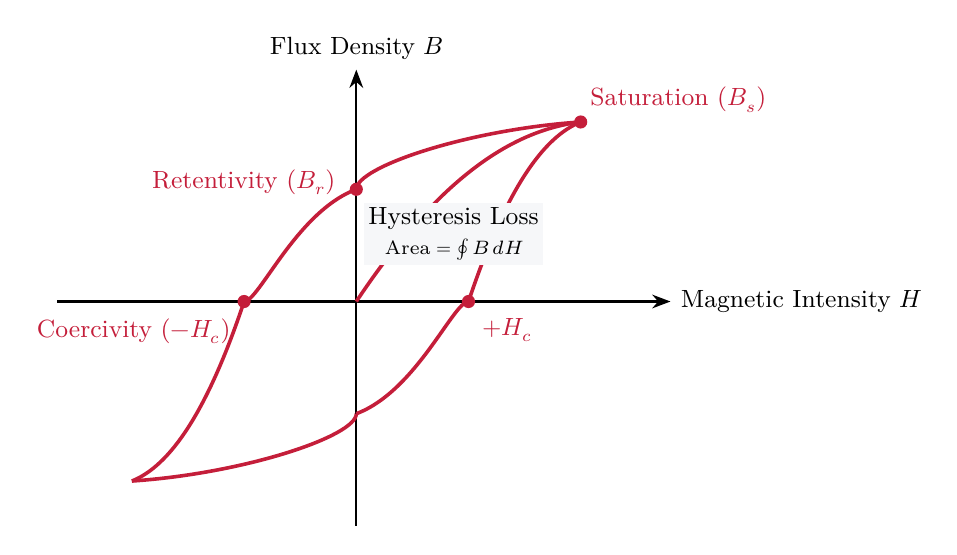
\begin{tikzpicture}[scale=0.95]
  % Axes
  \draw[-Stealth, thick] (-4,0) -- (4.2,0) node[right] {\small Magnetic Intensity $H$};
  \draw[-Stealth, thick] (0,-3) -- (0,3.1) node[above] {\small Flux Density $B$};
  
  % Hysteresis Loop
  \draw[myred, line width=1.3pt] (0,0) .. controls (1.2,1.8) and (2.2,2.3) .. (3,2.4);
  \draw[myred, line width=1.3pt] (3,2.4) .. controls (1.5,2.3) and (0,1.8) .. (0,1.5);
  \draw[myred, line width=1.3pt] (0,1.5) .. controls (-0.8,1.2) and (-1.3,0) .. (-1.5,0);
  \draw[myred, line width=1.3pt] (-1.5,0) .. controls (-2.0,-1.5) and (-2.5,-2.2) .. (-3,-2.4);
  \draw[myred, line width=1.3pt] (-3,-2.4) .. controls (-1.5,-2.3) and (0,-1.8) .. (0,-1.5);
  \draw[myred, line width=1.3pt] (0,-1.5) .. controls (0.8,-1.2) and (1.3,0) .. (1.5,0);
  \draw[myred, line width=1.3pt] (1.5,0) .. controls (2.0,1.5) and (2.5,2.2) .. (3,2.4);

  % Key Feature Markers & Labels
  \fill[myred] (3,2.4) circle (2.5pt);
  \node[myred, anchor=south west] at (3.0, 2.4) {\small Saturation ($B_s$)};

  \fill[myred] (0,1.5) circle (2.5pt);
  \node[myred, anchor=east] at (-0.15, 1.6) {\small Retentivity ($B_r$)};

  \fill[myred] (-1.5,0) circle (2.5pt);
  \node[myred, anchor=north east] at (-1.55, -0.1) {\small Coercivity ($-H_c$)};

  \fill[myred] (1.5,0) circle (2.5pt);
  \node[myred, anchor=north west] at (1.55, -0.1) {\small $+H_c$};

  % Hysteresis Loss text in clear region
  \node[align=center, fill=mygray, inner sep=1.5pt] at (1.3, 0.9) {\small Hysteresis Loss\\[-1pt]\scriptsize $\text{Area} = \oint B \, dH$};
\end{tikzpicture}
\end{tcolorbox}

\begin{tcolorbox}[defbox, title={\textbf{Hysteresis Terminology}}]
\begin{itemize}[leftmargin=*, itemsep=2pt]
  \item \textbf{Retentivity (Remanence $B_r$):} Residual flux density remaining in material when magnetising field $H$ is reduced to zero.
  \item \textbf{Coercivity ($H_c$):} Reverse magnetising field required to reduce residual flux density $B$ to zero.
  \item \textbf{Hysteresis Loss:} Energy dissipated per unit volume per cycle as heat during magnetisation reversal, equal to area enclosed by $B$-$H$ loop: $W_{\text{loss}} = \oint B \, dH$.
\end{itemize}
\end{tcolorbox}

\textbf{Soft vs. Hard Magnetic Materials:}\par\vspace{6pt}\noindent
\begin{tabularx}{\linewidth}{|B{3.2cm}|Y|Y|}
\hline
\textbf{Feature} & \textbf{Soft Magnetic Materials} & \textbf{Hard Magnetic Materials} \\
\hline
\textbf{Hysteresis Area} & Thin and narrow loop (low energy loss). & Broad and wide loop (high energy loss). \\
\hline
\textbf{Coercivity} & Very low coercivity ($H_c$ small). & Very high coercivity ($H_c$ large). \\
\hline
\textbf{Retentivity} & High retentivity, easily demagnetised. & High retentivity, retains magnetisation. \\
\hline
\textbf{Applications} & Transformer cores, electromagnets, inductors. & Permanent magnets, magnetic recording tapes, loudspeakers. \\
\hline
\end{tabularx}

\begin{tcolorbox}[examplebox, title={\textbf{Solved Problem 2: Hysteresis Loss Power Dissipation}}]
\textbf{Problem:} An iron ring of volume $V = 100\text{ cm}^3$ is subjected to a $50\text{ Hz}$ alternating magnetic field. If the area of the hysteresis loop corresponds to $250\text{ J/m}^3$ per cycle, calculate the power loss in watts.

\textbf{Solution:}\par\noindent
\begin{enumerate}[leftmargin=*, itemsep=2pt]
  \item Volume $V = 100 \times 10^{-6}\text{ m}^3 = 10^{-4}\text{ m}^3$.
  \item Frequency $f = 50\text{ Hz}$ (50 cycles/second).
  \item Energy loss per second (Power $P$) = Energy/cycle/volume $\times$ Volume $\times$ Frequency:
   \begin{equation}
   P = W_{\text{loss}} \times V \times f = 250\text{ J/m}^3 \times 10^{-4}\text{ m}^3 \times 50\text{ s}^{-1} = \mathbf{1.25\text{ W}}
   \end{equation}
\end{enumerate}
\end{tcolorbox}

% =============================================================================
% QUICK REVISION PAGE
% =============================================================================
\newpage
\begin{center}
  {\large\bfseries\color{myred} Quick Revision --- Module 3}\\[3pt]
  {\small\color{mydark} Electromagnetism \& Materials $|$ BS-PH101}
\end{center}
\noindent{\color{myred}\rule{\linewidth}{1.2pt}}
\vspace{4pt}

\begin{tcolorbox}[formulabox, title={\textbf{Key Formulas and Metrics at a Glance}}]
\renewcommand{\arraystretch}{1.35}
\begin{tabularx}{\linewidth}{B{5.0cm} X}
Maxwell 1 (Gauss Electro) & $\nabla \cdot \vec{D} = \rho \iff \oint_S \vec{D} \cdot d\vec{A} = Q_{\text{enclosed}}$ \\[4pt]
Maxwell 2 (Gauss Magneto) & $\nabla \cdot \vec{B} = 0 \iff \oint_S \vec{B} \cdot d\vec{A} = 0$ \\[4pt]
Maxwell 3 (Faraday) & $\nabla \times \vec{E} = -\frac{\partial \vec{B}}{\partial t} \iff \oint_C \vec{E} \cdot d\vec{r} = -\frac{\partial\Phi_B}{\partial t}$ \\[4pt]
Maxwell 4 (Ampere-Maxwell) & $\nabla \times \vec{H} = \vec{J} + \frac{\partial \vec{D}}{\partial t}$ \\[4pt]
Displacement Current & $\vec{J}_d = \frac{\partial \vec{D}}{\partial t} = \epsilon_0 \frac{\partial \vec{E}}{\partial t}$ \\[4pt]
Speed of Light in Vacuum & $c = \frac{1}{\sqrt{\mu_0 \epsilon_0}} = 3 \times 10^8\text{ m/s}$ \\[4pt]
Poynting Vector & $\vec{S} = \vec{E} \times \vec{H} \quad (\text{W/m}^2)$ \\[4pt]
Clausius-Mossotti Eq. & $\frac{\epsilon_r - 1}{\epsilon_r + 2} = \frac{N \alpha}{3 \epsilon_0}$ \\[4pt]
Magnetic Relations & $\vec{B} = \mu_0(\vec{H} + \vec{M})$ \quad and \quad $\mu_r = 1 + \chi_m$ \\[4pt]
Hysteresis Power Loss & $P_{\text{loss}} = (\oint B dH) \times \text{Volume} \times \text{Frequency}$ \\[4pt]
\end{tabularx}
\end{tcolorbox}

\begin{tcolorbox}[defbox, title={\textbf{One-Line Definitions}}]
\begin{itemize}[leftmargin=*, itemsep=2pt]
  \item \textbf{Displacement Current:} A quantity appearing in Maxwell's equations defined by rate of change of electric displacement field ($\vec{J}_d = \partial\vec{D}/\partial t$).
  \item \textbf{Poynting Vector:} A vector representing the directional energy flux density of an electromagnetic field ($\vec{S} = \vec{E} \times \vec{H}$).
  \item \textbf{Lorentz Local Field:} The actual local electric field acting at the position of an individual atom in a solid ($E_{\text{local}} = E + P/3\epsilon_0$).
  \item \textbf{Retentivity ($B_r$):} Residual magnetic flux density remaining in a ferromagnetic material when magnetising field $H$ is reduced to zero.
  \item \textbf{Coercivity ($H_c$):} The magnitude of reverse magnetic field intensity required to reduce residual magnetisation to zero.
\end{itemize}
\end{tcolorbox}

\begin{tcolorbox}[exambox, title={\textbf{Frequently Asked / Viva Questions}}]
\begin{enumerate}[topsep=0pt, label=\textbf{Q\arabic*.}, itemsep=5pt]
  \item \Q{Why did Maxwell modify Ampere's law and what term did he add?}
  Ampere's law ($\nabla \times \vec{H} = \vec{J}$) violated charge conservation for time-varying fields ($\nabla \cdot \vec{J} \neq 0$). Maxwell added displacement current density $\vec{J}_d = \partial\vec{D}/\partial t$.

  \item \Q{What is the physical significance of $\nabla \cdot \vec{B} = 0$?}
  It signifies that isolated magnetic monopoles do not exist in nature and magnetic flux lines always form continuous closed loops.

  \item \Q{What is Poynting vector and state its SI unit?}
  $\vec{S} = \vec{E} \times \vec{H}$ represents the rate of electromagnetic energy flow per unit area. Its SI unit is $\text{W/m}^2$.

  \item \Q{State the relation between dielectric constant $\epsilon_r$ and electric susceptibility $\chi_e$.}
  $\vec{D} = \epsilon_0 \vec{E} + \vec{P} = \epsilon_0(1 + \chi_e)\vec{E} = \epsilon_0 \epsilon_r \vec{E} \implies \epsilon_r = 1 + \chi_e$.

  \item \Q{Derive Clausius-Mossotti relation connecting macroscopic and microscopic dielectric properties.}
  Using Lorentz local field $E_{\text{local}} = E + P/3\epsilon_0$, total polarisation $P = N\alpha E_{\text{local}} = N\alpha(E + P/3\epsilon_0)$. Substituting $P = (\epsilon_r - 1)\epsilon_0 E$ yields $\frac{\epsilon_r - 1}{\epsilon_r + 2} = \frac{N\alpha}{3\epsilon_0}$.

  \item \Q{Distinguish between polar and non-polar dielectrics.}
  Polar dielectrics have permanent molecular dipole moments (e.g. $\text{H}_2\text{O}, \text{HCl}$); non-polar dielectrics have zero permanent dipole moment in zero field (e.g. $\text{O}_2, \text{N}_2, \text{CO}_2$).

  \item \Q{Why does orientational polarizability decrease with increasing temperature?}
  Because higher thermal agitation randomizes the orientation of permanent molecular dipoles, opposing their alignment along the external field ($\alpha_o \propto 1/T$).

  \item \Q{Distinguish between diamagnetic and paramagnetic materials.}
  Diamagnetic materials have no permanent dipoles, negative susceptibility ($\chi_m < 0$), and are repelled by magnetic fields. Paramagnetic materials have permanent dipoles, positive susceptibility ($\chi_m > 0$), and are feebly attracted.

  \item \Q{State Curie-Weiss law for ferromagnetic materials.}
  Above the Curie temperature $T_c$, a ferromagnetic material becomes paramagnetic with susceptibility $\chi_m = \frac{C}{T - T_c}$.

  \item \Q{What is meant by hysteresis loop area?}
  The area enclosed by the $B$-$H$ loop represents the energy dissipated as heat per unit volume per magnetization reversal cycle ($W_{\text{loss}} = \oint B \, dH$).

  \item \Q{Which magnetic material is suitable for transformer cores and why?}
  Soft magnetic materials (e.g. Soft Iron, Silicon Steel) because they have low coercivity and thin hysteresis loops, minimizing energy loss per cycle.

  \item \Q{Show that speed of EM wave in vacuum is $c = 1/\sqrt{\mu_0\epsilon_0}$.}
  From Maxwell's free-space wave equation $\nabla^2 \vec{E} = \mu_0\epsilon_0 \frac{\partial^2\vec{E}}{\partial t^2}$, comparing with standard wave equation $\nabla^2\psi = \frac{1}{v^2}\frac{\partial^2\psi}{\partial t^2}$ yields $v = c = 1/\sqrt{\mu_0\epsilon_0} \approx 3 \times 10^8\text{ m/s}$.
\end{enumerate}
\end{tcolorbox}

\begin{tcolorbox}[tikzbox, title={Summary Comparison of Dielectric Polarization Mechanisms}]
\centering
\begin{tabularx}{\linewidth}{|B{3.2cm}|Y|Y|Y|}
\hline
\textbf{Mechanism} & \textbf{Displacement Type} & \textbf{Frequency Range} & \textbf{Temperature Dependence} \\
\hline
\textbf{Electronic ($\alpha_e$)} & Electron cloud relative to nucleus. & Optical ($\sim 10^{15}\text{ Hz}$). & Independent of $T$. \\
\hline
\textbf{Ionic ($\alpha_i$)} & Positive and negative ion displacement. & Infrared ($\sim 10^{13}\text{ Hz}$). & Independent of $T$. \\
\hline
\textbf{Orientational ($\alpha_o$)} & Alignment of permanent dipoles. & Microwave ($\sim 10^{9}\text{ Hz}$). & Inverse with $T$ ($\alpha_o \propto 1/T$). \\
\hline
\textbf{Space-Charge ($\alpha_s$)} & Migration of charge carriers. & Audio ($\sim 10^{3}\text{ Hz}$). & Complex $T$ dependence. \\
\hline
\end{tabularx}
\end{tcolorbox}


% -- Module 4 -----------------------------------------------------------------
\modulestart{4}{Inadequacy of Classical Physics and Black Body Radiation}

\section{Inadequacy of Classical Physics and Black Body Radiation}

\subsection{Failure of Classical Mechanics and Planck's Radiation Law}

Classical physics (Rayleigh-Jeans law $u(\nu)d\nu = \frac{8\pi \nu^2}{c^3} k_B T d\nu$) predicted that black body radiation energy density tends to infinity at short wavelengths ($\lambda \to 0$), known as the \textbf{Ultraviolet Catastrophe}.

\begin{tcolorbox}[defbox, title={\textbf{Planck's Quantum Hypothesis (1900)}}]
Black body cavity walls consist of atomic oscillators that absorb or emit electromagnetic radiation in discrete packets called \textbf{quanta} (photons) of energy:
\begin{equation}
E = n h \nu \quad (n = 1, 2, 3, \ldots)
\end{equation}
where $h = 6.626 \times 10^{-34}\text{ J}\cdot\text{s}$ is Planck's constant.
\end{tcolorbox}

\begin{tcolorbox}[formulabox, title={\textbf{Planck's Black Body Radiation Law Derivation}}]
Average energy of an oscillator $\langle E \rangle = \frac{\sum_{n=0}^\infty n h\nu \, e^{-n h\nu / k_B T}}{\sum_{n=0}^\infty e^{-n h\nu / k_B T}} = \frac{h\nu}{e^{h\nu / k_B T} - 1}$.
Multiplying by number of modes per unit volume $N(\nu)d\nu = \frac{8\pi \nu^2}{c^3} d\nu$:
\begin{equation}
u(\nu) d\nu = \frac{8\pi h \nu^3}{c^3} \frac{1}{e^{h\nu / k_B T} - 1} d\nu \iff u(\lambda) d\lambda = \frac{8\pi h c}{\lambda^5} \frac{1}{e^{hc / \lambda k_B T} - 1} d\lambda
\end{equation}
\end{tcolorbox}

\textbf{Deduction of Limiting Laws:}\par\noindent
\begin{itemize}[leftmargin=*, itemsep=3pt]
  \item \textbf{Rayleigh-Jeans Law (Long $\lambda$):} For $h\nu \ll k_B T$, $e^{h\nu/k_B T} - 1 \approx \frac{h\nu}{k_B T} \implies u(\nu)d\nu = \frac{8\pi \nu^2}{c^3} k_B T d\nu$.
  \item \textbf{Wien's Distribution Law (Short $\lambda$):} For $h\nu \gg k_B T$, $e^{h\nu/k_B T} - 1 \approx e^{h\nu/k_B T} \implies u(\lambda)d\lambda = \frac{8\pi hc}{\lambda^5} e^{-hc/\lambda k_B T} d\lambda$.
\end{itemize}

% =============================================================================
% SECTION 2: COMPTON EFFECT & MATTER WAVES
% =============================================================================
\section{Compton Effect, de Broglie Hypothesis, and Matter Waves}

\subsection{Compton Effect}

When a high-energy X-ray or $\gamma$-ray photon collides elastically with a stationary free electron, the scattered photon emerges with a longer wavelength ($\lambda' > \lambda$).

\begin{tcolorbox}[formulabox, title={\textbf{Derivation of Compton Shift Formula}}]
Applying conservation of relativistic energy and momentum during collision:
\begin{align}
\text{Energy Conservation: } & h\nu + m_0 c^2 = h\nu' + m c^2 \\[4pt]
\text{Momentum Conservation: } & \vec{p}_{\text{photon}} = \vec{p}'_{\text{photon}} + \vec{p}_{\text{electron}}
\end{align}
Eliminating electron velocity $v$ using $m = \frac{m_0}{\sqrt{1 - v^2/c^2}}$ yields the \textbf{Compton Shift Equation}:
\begin{equation}
\Delta \lambda = \lambda' - \lambda = \frac{h}{m_0 c} (1 - \cos\theta) = 2 \lambda_c \sin^2\left(\frac{\theta}{2}\right)
\end{equation}
where $\lambda_c = \frac{h}{m_0 c} = 0.02426\text{ \AA} = 2.426 \times 10^{-12}\text{ m}$ is the \textbf{Compton Wavelength}.
\end{tcolorbox}

\textbf{Key Characteristics of Compton Shift:}
\begin{itemize}[leftmargin=*, itemsep=2pt]
  \item $\Delta \lambda$ depends \textit{only} on scattering angle $\theta$, independent of incident wavelength or target material.
  \item Maximum shift occurs at $\theta = 180^\circ$ (backscattering): $\Delta \lambda_{\max} = \frac{2h}{m_0 c} = 0.0485\text{ \AA}$.
  \item Compton shift is absent for visible light because $\Delta\lambda \ll \lambda_{\text{visible}}$ is unresolvable.
\end{itemize}

\begin{tcolorbox}[tikzbox, title={Compton Scattering Geometry}]
\centering
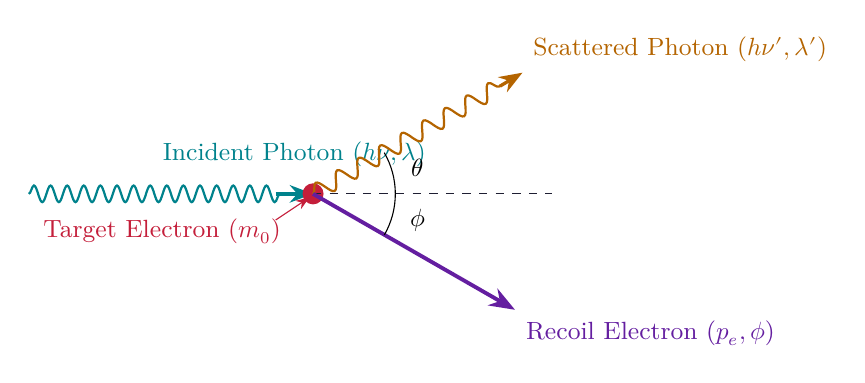
\begin{tikzpicture}[scale=0.95]
  % Incident Photon Wave
  \draw[thick, myteal, decorate, decoration={snake, segment length=6pt, amplitude=3pt}] (-3.8,0) -- (-0.4,0);
  \draw[-Stealth, line width=1.2pt, myteal] (-0.5,0) -- (0,0) node[midway, above=6pt] {\small Incident Photon ($h\nu, \lambda$)};
  
  % Target Electron
  \fill[myred] (0,0) circle (4pt);
  \node[myred, anchor=east] at (-0.3,-0.5) {\small Target Electron ($m_0$)};
  \draw[-Stealth, thin, myred] (-0.5,-0.35) -- (-0.05,-0.05);
  
  % Dashed baseline
  \draw[dashed, mydark] (0,0) -- (3.2,0);

  % Scattered Photon Wave
  \draw[thick, myamber, decorate, decoration={snake, segment length=9pt, amplitude=3pt}] (0,0) -- (2.6, 1.5);
  \draw[-Stealth, line width=1.2pt, myamber] (2.5, 1.44) -- (2.8, 1.62) node[above right] {\small Scattered Photon ($h\nu', \lambda'$)};
  \draw[thin] (1.1,0) arc (0:30:1.1);
  \node at (1.4,0.35) {\small $\theta$};
  
  % Recoil Electron
  \draw[-Stealth, line width=1.4pt, mypurple] (0,0) -- (2.7, -1.55) node[below right] {\small Recoil Electron ($p_e, \phi$)};
  \draw[thin] (1.1,0) arc (0:-30:1.1);
  \node at (1.4,-0.35) {\small $\phi$};
\end{tikzpicture}
\end{tcolorbox}

\subsection{de Broglie Hypothesis and Davisson-Germer Experiment}

\begin{tcolorbox}[defbox, title={\textbf{Definition: de Broglie Hypothesis}}]
Louis de Broglie (1924) proposed that moving matter particles exhibit wave properties with a wavelength ($\lambda$) inversely proportional to momentum ($p$):
\begin{equation}
\lambda = \frac{h}{p} = \frac{h}{m v} = \frac{h}{\sqrt{2m E}} = \frac{h}{\sqrt{2m q V}}
\end{equation}
For an electron accelerated through potential $V$ volts:
\begin{equation}
\lambda_e = \frac{12.27}{\sqrt{V}} \text{ \AA}
\end{equation}
\end{tcolorbox}

\textbf{Davisson-Germer Experiment:} Accelerated electrons at $V = 54\text{ V}$ onto a Nickel crystal target observed a pronounced scattering peak at angle $\phi = 50^\circ$.
Bragg diffraction angle $\theta = 90^\circ - \phi/2 = 65^\circ$.
\begin{equation}
\lambda_{\text{Bragg}} = 2 d \sin\theta = 2(0.91\text{ \AA}) \sin 65^\circ = \mathbf{1.65\text{ \AA}} \quad \text{vs} \quad \lambda_{\text{de Broglie}} = \frac{12.27}{\sqrt{54}} = \mathbf{1.67\text{ \AA}}
\end{equation}
This excellent agreement provided direct experimental verification of matter waves.

\begin{tcolorbox}[examplebox, title={\textbf{Solved Problem 1: Compton Shift at 90 Degrees}}]
\textbf{Problem:} X-rays of wavelength $\lambda = 1.0\text{ \AA}$ are scattered by a target at $\theta = 90^\circ$. Calculate: (a) Scattered wavelength $\lambda'$, (b) Energy of recoil electron.

\textbf{Solution:}\par\noindent
\begin{enumerate}[leftmargin=*, itemsep=2pt]
  \item $\Delta \lambda = \lambda_c (1 - \cos 90^\circ) = 0.02426\text{ \AA} (1 - 0) = 0.02426\text{ \AA}$.
  \item Scattered wavelength $\lambda' = \lambda + \Delta \lambda = 1.0 + 0.02426 = \mathbf{1.02426\text{ \AA}}$.
  \item Recoil electron kinetic energy $K_e = h c \left(\frac{1}{\lambda} - \frac{1}{\lambda'}\right) = h c \frac{\Delta\lambda}{\lambda \lambda'}$:
   \begin{equation}
   K_e = \frac{(6.626 \times 10^{-34}) (3 \times 10^8) (0.02426 \times 10^{-10})}{(1.0 \times 10^{-10}) (1.02426 \times 10^{-10})} = 4.706 \times 10^{-17}\text{ J} = \mathbf{294.1\text{ eV}}
   \end{equation}
\end{enumerate}
\end{tcolorbox}

% =============================================================================
% SECTION 3: HEISENBERG UNCERTAINTY PRINCIPLE
% =============================================================================
\section{Heisenberg Uncertainty Principle}

\subsection{Uncertainty Relations}

\begin{tcolorbox}[formulabox, title={\textbf{Heisenberg Uncertainty Principle Relations}}]
It is impossible to simultaneously measure both the exact position and exact momentum of a particle with absolute precision:
\begin{equation}
\Delta x \cdot \Delta p_x \ge \frac{\hbar}{2} \quad \left(\text{where } \hbar = \frac{h}{2\pi} = 1.054 \times 10^{-34} \text{ J}\cdot\text{s}\right)
\end{equation}
Alternate canonical conjugate forms:
\begin{align}
\text{Energy-Time Uncertainty: } & \Delta E \cdot \Delta t \ge \frac{\hbar}{2} \\[3pt]
\text{Angular Position-Momentum: } & \Delta \theta \cdot \Delta L_z \ge \frac{\hbar}{2}
\end{align}
\end{tcolorbox}

\subsection{Applications: Non-Existence of Electron in Nucleus}

\begin{tcolorbox}[examplebox, title={\textbf{Proof: Non-Existence of Electron in Nucleus}}]
\textbf{Premise:} Radius of atomic nucleus is $r \approx 5 \times 10^{-15}\text{ m}$. If an electron exists inside, maximum position uncertainty $\Delta x \approx 10^{-14}\text{ m}$.

\begin{enumerate}[leftmargin=*, itemsep=2pt]
  \item Minimum momentum uncertainty:
   \begin{equation}
   \Delta p \ge \frac{\hbar}{2 \Delta x} = \frac{1.054 \times 10^{-34}}{2 \times 10^{-14}} = 5.27 \times 10^{-21}\text{ kg}\cdot\text{m/s}
   \end{equation}
  \item Minimum relativistic energy of electron ($E \approx p c$ for $p \gg m_0 c$):
   \begin{equation}
   E_{\min} \approx \Delta p \cdot c = (5.27 \times 10^{-21}) \times (3 \times 10^8) = 1.58 \times 10^{-12}\text{ J} \approx \mathbf{9.9\text{ MeV}}
   \end{equation}
  \item Experimental $\beta$-decay electrons emitted from nucleus have maximum energies of only $2 - 3\text{ MeV}$.
\end{enumerate}
\textbf{Conclusion:} Electrons \textbf{cannot reside} inside the nucleus.
\end{tcolorbox}

% =============================================================================
% SECTION 4: SCHRÖDINGER WAVE EQUATION
% =============================================================================
\section{Schrödinger Wave Equation and Wave Function}

\subsection{Physical Interpretation of Wave Function \texorpdfstring{$\psi$}{psi}}

The wave function $\psi(\vec{r}, t)$ describes the quantum state of a particle.

\begin{tcolorbox}[defbox, title={\textbf{Born's Probability Interpretation of Wave Function}}]
$\psi$ itself is a complex quantity without direct physical measurement. However, the scalar product $|\psi(\vec{r},t)|^2 = \psi^* \psi$ represents the \textbf{probability density} of finding the particle at position $\vec{r}$ at time $t$.
\begin{equation}
P = \int_{-\infty}^{\infty} |\psi(x,t)|^2 dx = 1 \quad (\text{Normalization Condition})
\end{equation}
\end{tcolorbox}

\textbf{Criteria for an Acceptable Quantum Wave Function:}\par\noindent
\begin{enumerate}[leftmargin=*, itemsep=2pt]
  \item $\psi$ must be \textbf{single-valued} at all points in space.
  \item $\psi$ and its spatial derivative $\frac{\partial\psi}{\partial x}$ must be \textbf{continuous} everywhere.
  \item $\psi$ must be \textbf{square-integrable} (normalizable, $\psi \to 0$ as $r \to \infty$).
\end{enumerate}

\subsection{Time-Dependent and Time-Independent Schrödinger Equations}

\begin{tcolorbox}[formulabox, title={\textbf{Schrödinger Wave Equations}}]
\begin{itemize}[leftmargin=*, itemsep=4pt]
  \item \textbf{1D Time-Dependent Schrödinger Equation:}
  \begin{equation}
  -\frac{\hbar^2}{2m} \frac{\partial^2 \psi(x,t)}{\partial x^2} + V(x,t)\psi(x,t) = i\hbar \frac{\partial \psi(x,t)}{\partial t}
  \end{equation}
  \item \textbf{1D Time-Independent Schrödinger Equation} (for stationary states $\psi(x,t) = \psi(x) e^{-i E t / \hbar}$):
  \begin{equation}
  \frac{d^2 \psi(x)}{dx^2} + \frac{2m}{\hbar^2}\big(E - V(x)\big)\psi(x) = 0 \iff \hat{H}\psi = E\psi
  \end{equation}
  where $\hat{H} = -\frac{\hbar^2}{2m}\nabla^2 + V$ is the Hamiltonian operator.
\end{itemize}
\end{tcolorbox}

% =============================================================================
% SECTION 5: QUANTUM APPLICATIONS
% =============================================================================
\section{Quantum Applications: Particle in Box, Harmonic Oscillator, H-Atom}

\subsection{Particle in a 1D Infinite Potential Box}

Consider a particle of mass $m$ confined in a 1D box of length $L$ ($V(x) = 0$ for $0 < x < L$, and $V(x) = \infty$ outside).

Inside the box ($0 < x < L$), $\frac{d^2\psi}{dx^2} + k^2 \psi = 0$ where $k = \frac{\sqrt{2mE}}{\hbar}$.
Boundary conditions $\psi(0) = 0$ and $\psi(L) = 0$ require $k L = n \pi$.

\begin{tcolorbox}[formulabox, title={\textbf{1D Box Eigenvalues and Normalised Eigenfunctions}}]
\begin{align}
\text{Energy Eigenvalues: } & E_n = \frac{n^2 \pi^2 \hbar^2}{2 m L^2} = \frac{n^2 h^2}{8 m L^2} \quad (n = 1, 2, 3, \ldots) \\[4pt]
\text{Normalised Wavefunctions: } & \psi_n(x) = \sqrt{\frac{2}{L}} \sin\left(\frac{n \pi x}{L}\right)
\end{align}
\end{tcolorbox}

\textbf{Key Consequences:}\par\noindent
\begin{itemize}[leftmargin=*, itemsep=2pt]
  \item \textbf{Energy Quantization:} Energy levels are discrete and proportional to $n^2$.
  \item \textbf{Zero-Point Energy ($E_1$):} The lowest possible energy is $E_1 = \frac{h^2}{8mL^2} \neq 0$, agreeing with uncertainty principle.
  \item \textbf{Degeneracy in 3D Cubic Box:} $E_{n_x,n_y,n_z} = \frac{h^2}{8mL^2}(n_x^2 + n_y^2 + n_z^2)$. States with different quantum numbers sharing same energy are \textbf{degenerate} (e.g. $(1,1,2), (1,2,1), (2,1,1)$ is 3-fold degenerate).
\end{itemize}

\subsection{Quantum Harmonic Oscillator and Hydrogen Atom}

\begin{tcolorbox}[formulabox, title={\textbf{Quantum Harmonic Oscillator and Hydrogen Atom Energies}}]
\begin{itemize}[leftmargin=*, itemsep=4pt]
  \item \textbf{Quantum Harmonic Oscillator ($V = \frac{1}{2}m\omega^2 x^2$):}
  \begin{equation}
  E_n = \left(n + \frac{1}{2}\right)\hbar \omega \quad (n = 0, 1, 2, \ldots)
  \end{equation}
  Zero-point energy $E_0 = \frac{1}{2}\hbar \omega$ (unlike classical oscillator which can rest at zero energy).
  \item \textbf{Hydrogen Atom (Coulomb Potential $V = -\frac{e^2}{4\pi\epsilon_0 r}$):}
  \begin{equation}
  E_n = -\frac{m e^4}{32 \pi^2 \epsilon_0^2 \hbar^2 n^2} = -\frac{13.6}{n^2} \text{ eV} \quad (n = 1, 2, 3, \ldots)
  \end{equation}
  Described by four quantum numbers: Principal ($n$), Orbital ($l$), Magnetic ($m_l$), and Spin ($m_s$).
\end{itemize}
\end{tcolorbox}

\begin{tcolorbox}[examplebox, title={\textbf{Solved Problem 2: Particle in 1D Box Transition Energy}}]
\textbf{Problem:} An electron is trapped in a 1D infinite box of width $L = 1.0\text{ \AA}$. Calculate: (a) Ground state energy $E_1$ in eV, (b) Wavelength of photon emitted during transition from $n=2 \to n=1$.

\textbf{Solution:}\par\noindent
\begin{enumerate}[leftmargin=*, itemsep=2pt]
  \item Ground state energy $E_1 = \frac{h^2}{8 m L^2}$:
   \begin{equation}
   E_1 = \frac{(6.626 \times 10^{-34})^2}{8 \times (9.11 \times 10^{-31}) \times (1.0 \times 10^{-10})^2} = 6.025 \times 10^{-18}\text{ J} = \mathbf{37.66\text{ eV}}
   \end{equation}
  \item First excited energy $E_2 = 2^2 E_1 = 4 (37.66) = 150.64\text{ eV}$.
  \item Energy difference $\Delta E = E_2 - E_1 = 3 E_1 = 112.98\text{ eV} = 1.808 \times 10^{-17}\text{ J}$.
  \item Emitted wavelength $\lambda = \frac{h c}{\Delta E} = \frac{(6.626 \times 10^{-34}) (3 \times 10^8)}{1.808 \times 10^{-17}} = 1.10 \times 10^{-8}\text{ m} = \mathbf{110\text{ \AA}}$.
\end{enumerate}
\end{tcolorbox}

% =============================================================================
% QUICK REVISION PAGE
% =============================================================================
\newpage
\begin{center}
  {\large\bfseries\color{myred} Quick Revision --- Module 4}\\[3pt]
  {\small\color{mydark} Quantum Mechanics $|$ BS-PH101}
\end{center}
\noindent{\color{myred}\rule{\linewidth}{1.2pt}}
\vspace{4pt}

\begin{tcolorbox}[formulabox, title={\textbf{Key Formulas and Metrics at a Glance}}]
\renewcommand{\arraystretch}{1.35}
\begin{tabularx}{\linewidth}{B{5.0cm} X}
Planck Photon Energy & $E = h \nu = \frac{hc}{\lambda}$ \\[4pt]
Planck Radiation Law & $u(\lambda)d\lambda = \frac{8\pi h c}{\lambda^5} \frac{1}{e^{hc/\lambda k_B T} - 1} d\lambda$ \\[4pt]
Compton Shift Equation & $\Delta\lambda = \lambda' - \lambda = \frac{h}{m_0 c}(1 - \cos\theta)$ \\[4pt]
Compton Wavelength & $\lambda_c = \frac{h}{m_0 c} = 0.02426\text{ \AA}$ \\[4pt]
de Broglie Wavelength & $\lambda = \frac{h}{p} = \frac{12.27}{\sqrt{V}}\text{ \AA} \quad (\text{for electron})$ \\[4pt]
Heisenberg Uncertainty & $\Delta x \cdot \Delta p \ge \frac{\hbar}{2} \quad \text{and} \quad \Delta E \cdot \Delta t \ge \frac{\hbar}{2}$ \\[4pt]
1D Time-Indep. Schrödinger & $\frac{d^2\psi}{dx^2} + \frac{2m}{\hbar^2}(E - V)\psi = 0$ \\[4pt]
1D Box Energy Eigenvalue & $E_n = \frac{n^2 h^2}{8 m L^2} \quad (n = 1, 2, 3, \ldots)$ \\[4pt]
1D Box Wavefunction & $\psi_n(x) = \sqrt{\frac{2}{L}} \sin\left(\frac{n\pi x}{L}\right)$ \\[4pt]
Harmonic Oscillator Energy & $E_n = (n + 1/2)\hbar \omega \quad (\text{Zero-point } E_0 = \frac{1}{2}\hbar\omega)$ \\[4pt]
Hydrogen Atom Energy & $E_n = -\frac{13.6}{n^2}\text{ eV}$ \\[4pt]
\end{tabularx}
\end{tcolorbox}

\begin{tcolorbox}[defbox, title={\textbf{One-Line Definitions}}]
\begin{itemize}[leftmargin=*, itemsep=2pt]
  \item \textbf{Compton Effect:} The increase in wavelength of X-ray/$\gamma$-ray photons when scattered by weakly bound target electrons.
  \item \textbf{Wave-Particle Duality:} The property of matter and light exhibiting both wave-like and particle-like behaviors depending on experimental setup.
  \item \textbf{Probability Density ($|\psi|^2$):} The probability per unit volume of finding a quantum particle at a specific spatial coordinate.
  \item \textbf{Zero-Point Energy:} The lowest possible non-zero ground-state energy that a quantum mechanical physical system may possess ($E_1 \neq 0$).
  \item \textbf{Degeneracy:} The phenomenon where two or more distinct quantum states share the exact same energy eigenvalue.
\end{itemize}
\end{tcolorbox}

\begin{tcolorbox}[exambox, title={\textbf{Frequently Asked / Viva Questions}}]
\begin{enumerate}[topsep=0pt, label=\textbf{Q\arabic*.}, itemsep=5pt]
  \item \Q{What was Rayleigh-Jeans law and why did it fail?}
  Rayleigh-Jeans law ($u(\nu) \propto \nu^2 T$) predicted infinite energy density at high frequencies ($\lambda \to 0$), causing the ultraviolet catastrophe.

  \item \Q{State Planck's quantum hypothesis.}
  Atomic oscillators absorb or emit electromagnetic radiation only in discrete energy quanta $E = n h \nu$.

  \item \Q{Why does Compton effect observe no shift at $\theta = 0^\circ$ and maximum shift at $\theta = 180^\circ$?}
  $\Delta\lambda = \lambda_c (1 - \cos\theta)$. At $\theta = 0^\circ$, $\cos 0^\circ = 1 \implies \Delta\lambda = 0$. At $\theta = 180^\circ$, $\cos 180^\circ = -1 \implies \Delta\lambda = 2\lambda_c = 0.0485\text{ \AA}$.

  \item \Q{Why is Compton effect not observable with visible light?}
  Visible light has wavelength $\sim 5000\text{ \AA}$. The maximum Compton shift ($0.0485\text{ \AA}$) is less than $0.001\%$ of $\lambda_{\text{visible}}$ and cannot be resolved.

  \item \Q{What is de Broglie wavelength of an electron accelerated through $V$ volts?}
  $\lambda = \frac{h}{\sqrt{2m q V}} = \frac{12.27}{\sqrt{V}}\text{ \AA}$.

  \item \Q{Explain the physical significance of Davisson-Germer experiment.}
  It demonstrated electron diffraction from a Nickel crystal lattice, proving experimentally that moving material particles possess wave characteristics.

  \item \Q{Prove using uncertainty principle that electron cannot reside inside atomic nucleus.}
  For nuclear radius $\Delta x \approx 10^{-14}\text{ m}$, $\Delta p \ge \hbar / 2\Delta x \implies E \approx \Delta p \cdot c \approx 9.9\text{ MeV}$. Experimental $\beta$-decay energies are only $2-3\text{ MeV}$, proving electrons cannot reside in nucleus.

  \item \Q{State Born's physical interpretation of wave function $\psi$.}
  $\psi$ itself has no direct physical measurement, but $|\psi(\vec{r},t)|^2 = \psi^* \psi$ represents the probability density of finding the particle at $\vec{r}$ at time $t$.

  \item \Q{What are the mandatory conditions for an acceptable wave function?}
  $\psi$ must be single-valued, continuous everywhere along with its first spatial derivative, and square-integrable ($\int |\psi|^2 dV = 1$).

  \item \Q{Why is ground state energy of particle in 1D box non-zero?}
  If $E_1 = 0 \implies p = 0 \implies \Delta p = 0$, requiring $\Delta x = \infty$ by uncertainty principle, contradicting confinement in box of finite length $L$.

  \item \Q{What is zero-point energy of a quantum harmonic oscillator?}
  $E_0 = \frac{1}{2}\hbar \omega$. Unlike classical oscillators, quantum oscillators retain non-zero vibrational energy even at absolute zero temperature ($T = 0\text{ K}$).

  \item \Q{What is meant by degeneracy of energy levels?}
  Degeneracy occurs when multiple independent quantum wavefunctions (different sets of quantum numbers) correspond to the exact same energy eigenvalue (e.g. $(1,1,2), (1,2,1), (2,1,1)$ in a 3D box).
\end{enumerate}
\end{tcolorbox}

\begin{tcolorbox}[tikzbox, title={Summary Comparison of Quantum Models}]
\centering
\begin{tabularx}{\linewidth}{|B{3.2cm}|Y|Y|Y|}
\hline
\textbf{System Model} & \textbf{Potential $V(x)$} & \textbf{Ground State Energy ($E_1$ or $E_0$)} & \textbf{Energy Spacing ($\Delta E$)} \\
\hline
\textbf{Particle in 1D Box} & $V=0$ ($0<x<L$), $V=\infty$ outside & $E_1 = \frac{h^2}{8mL^2}$ & Non-uniform ($\propto n^2$). \\
\hline
\textbf{Harmonic Oscillator} & $V = \frac{1}{2}m\omega^2 x^2$ & $E_0 = \frac{1}{2}\hbar\omega$ & Uniform ($\Delta E = \hbar\omega$). \\
\hline
\textbf{Hydrogen Atom} & $V = -\frac{e^2}{4\pi\epsilon_0 r}$ & $E_1 = -13.6\text{ eV}$ & Concentrated near continuum ($\propto -1/n^2$). \\
\hline
\end{tabularx}
\end{tcolorbox}


% -- Module 5 -----------------------------------------------------------------
\modulestart{5}{Macrostate, Microstate, Phase Space, and Ensembles}

\section{Macrostate, Microstate, Phase Space, and Ensembles}

\subsection{Basic Concepts of Statistical Mechanics}

Statistical mechanics connects the microscopic behavior of individual atoms/molecules with the macroscopic thermodynamic properties ($P, V, T, S$) of a system.

\begin{tcolorbox}[defbox, title={\textbf{Definitions: Macrostate, Microstate, and Phase Space}}]
\begin{itemize}[leftmargin=*, itemsep=2pt]
  \item \textbf{Macrostate:} The macroscopic state of a system specified by overall thermodynamic variables (e.g. $(N, V, E)$ or $(N, V, T)$).
  \item \textbf{Microstate:} A specific detailed configuration of the system specifying the exact position ($\vec{r}_i$) and momentum ($\vec{p}_i$) of every individual particle.
  \item \textbf{Phase Space:} A $6N$-dimensional conceptual space formed by 3 position coordinates $(x,y,z)$ and 3 momentum coordinates $(p_x,p_y,p_z)$ for each of $N$ particles. The elementary phase cell volume in quantum mechanics is $h^3$.
  \item \textbf{Thermodynamic Probability ($W$):} The total number of microstates corresponding to a given macrostate.
\end{itemize}
\end{tcolorbox}

\begin{tcolorbox}[formulabox, title={\textbf{Boltzmann Entropy Relation}}]
\begin{equation}
S = k_B \ln W
\end{equation}
where $k_B = 1.38 \times 10^{-23}\text{ J/K}$ is Boltzmann's constant, and $W$ is the thermodynamic probability.
\end{tcolorbox}

\subsection{Statistical Ensembles}

An \textbf{ensemble} is a large collection of independent, macroscopically identical systems existing in different microstates.

\textbf{Three Main Gibbs Ensembles:}\par\vspace{6pt}\noindent
\begin{tabularx}{\linewidth}{|B{3.2cm}|Y|Y|}
\hline
\textbf{Ensemble} & \textbf{Fixed Parameters} & \textbf{Physical System Example} \\
\hline
\textbf{Microcanonical} & Number $N$, Volume $V$, Energy $E$ (Rigid, isolated, insulated walls). & Isolated system with zero heat exchange. \\
\hline
\textbf{Canonical} & Number $N$, Volume $V$, Temperature $T$ (Diathermal walls in heat bath). & Closed system exchanging heat with a reservoir. \\
\hline
\textbf{Grand Canonical} & Chem. potential $\mu$, Volume $V$, Temp. $T$ (Permeable, diathermal walls). & Open system exchanging both energy and particles. \\
\hline
\end{tabularx}

\begin{tcolorbox}[examplebox, title={\textbf{Solved Problem 1: Microstates and Entropy}}]
\textbf{Problem:} Calculate the number of microstates and thermodynamic probability $W$ for distributing $N = 4$ distinguishable particles in 2 equal compartments. Find the entropy of the most probable state.

\textbf{Solution:}\par\noindent
\begin{enumerate}[leftmargin=*, itemsep=2pt]
  \item Total number of microstates = $2^N = 2^4 = \mathbf{16}$.
  \item Macrostates are given by $(n_1, n_2)$ where $n_1 + n_2 = 4$:
  \begin{itemize}[leftmargin=*, itemsep=1pt]
    \item $(4,0): W = \frac{4!}{4!0!} = 1$
    \item $(3,1): W = \frac{4!}{3!1!} = 4$
    \item $(2,2): W = \frac{4!}{2!2!} = \mathbf{6} \quad (\text{Most Probable Macrostate})$
    \item $(1,3): W = 4$
    \item $(0,4): W = 1$
  \end{itemize}
  \item Entropy of most probable macrostate $(2,2)$:
   \begin{equation}
   S = k_B \ln(6) = (1.38 \times 10^{-23}) \times 1.7917 = \mathbf{2.47 \times 10^{-23}\text{ J/K}}
   \end{equation}
\end{enumerate}
\end{tcolorbox}

% =============================================================================
% SECTION 2: DENSITY OF STATES
% =============================================================================
\section{Density of States}

\subsection{Derivation of Density of States in 3D}

The \textbf{Density of States ($g(E)dE$)} represents the number of available quantum states per unit volume in the energy range between $E$ and $E + dE$.

\begin{tcolorbox}[formulabox, title={\textbf{3D Free Particle Density of States Derivation}}]
In momentum space, momentum $p = \sqrt{2mE}$. The volume of momentum sphere of radius $p$ is $V_p = \frac{4}{3}\pi p^3 = \frac{4}{3}\pi (2mE)^{3/2}$.
The number of spatial-momentum phase cells of volume $h^3$ inside spatial volume $V$ is:
\begin{equation}
N(E) = \frac{V \cdot \frac{4}{3}\pi (2mE)^{3/2}}{h^3} = \frac{4\pi V (2m)^{3/2}}{3 h^3} E^{3/2}
\end{equation}
Taking the derivative with respect to $E$ gives $g(E) = \frac{dN(E)}{dE}$:
\begin{equation}
g(E) dE = \frac{4\pi V (2m)^{3/2}}{h^3} E^{1/2} dE
\end{equation}
Including electron spin degeneracy $g_s = 2s+1 = 2$ for electrons:
\begin{equation}
g_e(E) dE = \frac{8\pi V (2m)^{3/2}}{h^3} E^{1/2} dE
\end{equation}
\end{tcolorbox}

\textbf{Density of States in Lower Dimensions:}\par\noindent
\begin{enumerate}[leftmargin=*, itemsep=2pt]
  \item \textbf{1D System:} $g_{1D}(E) \propto E^{-1/2}$.
  \item \textbf{2D System:} $g_{2D}(E) = \text{constant}$ (independent of energy $E$).
  \item \textbf{3D System:} $g_{3D}(E) \propto E^{1/2}$.
\end{enumerate}

\begin{tcolorbox}[tikzbox, title={Density of States $g(E)$ in 1D, 2D, and 3D Systems}]
\centering
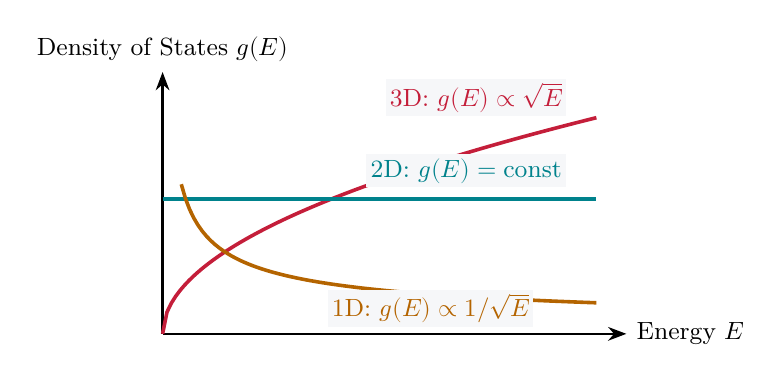
\begin{tikzpicture}[scale=0.95]
  % Axes
  \draw[-Stealth, thick] (0,0) -- (6.2,0) node[right] {\small Energy $E$};
  \draw[-Stealth, thick] (0,0) -- (0,3.5) node[above] {\small Density of States $g(E)$};

  % 3D Curve (Square root)
  \draw[myred, line width=1.3pt, domain=0:5.8, samples=100] plot (\x, {1.2*sqrt(\x)});
  \node[myred, fill=mygray, inner sep=1.5pt, anchor=south east] at (5.4, 2.9) {\small 3D: $g(E) \propto \sqrt{E}$};

  % 2D Curve (Constant)
  \draw[myteal, line width=1.3pt, domain=0:5.8] plot (\x, {1.8});
  \node[myteal, fill=mygray, inner sep=1.5pt, anchor=south east] at (5.4, 1.95) {\small 2D: $g(E) = \text{const}$};

  % 1D Curve (1/sqrt)
  \draw[myamber, line width=1.3pt, domain=0.25:5.8, samples=100] plot (\x, {1.0/sqrt(\x)});
  \node[myamber, fill=mygray, inner sep=1.5pt, anchor=north west] at (2.2, 0.6) {\small 1D: $g(E) \propto 1/\sqrt{E}$};
\end{tikzpicture}
\end{tcolorbox}

% =============================================================================
% SECTION 3: CLASSICAL AND QUANTUM STATISTICS
% =============================================================================
\section{Maxwell-Boltzmann, Bose-Einstein, and Fermi-Dirac Statistics}

\subsection{Qualitative and Quantitative Treatment}

Depending on particle distinguishability, quantum spin, and wave function symmetry:

\begin{tcolorbox}[formulabox, title={\textbf{Three Distribution Functions}}]
\begin{itemize}[leftmargin=*, itemsep=3pt]
  \item \textbf{Maxwell-Boltzmann (MB):} Classical, distinguishable particles, no spin restriction:
  \begin{equation}
  f_{\text{MB}}(E) = A e^{-E / k_B T}
  \end{equation}
  \item \textbf{Bose-Einstein (BE):} Quantum, indistinguishable particles with integer spin ($s=0, 1, 2, \ldots$, Bosons):
  \begin{equation}
  f_{\text{BE}}(E) = \frac{1}{e^{(E-\mu)/k_B T} - 1}
  \end{equation}
  \item \textbf{Fermi-Dirac (FD):} Quantum, indistinguishable particles with half-integer spin ($s=1/2, 3/2, \ldots$, Fermions), obeys Pauli Exclusion Principle:
  \begin{equation}
  f_{\text{FD}}(E) = \frac{1}{e^{(E-E_F)/k_B T} + 1}
  \end{equation}
\end{itemize}
\end{tcolorbox}

\textbf{Comprehensive 8-Criterion Comparison Table:}\par\vspace{6pt}\noindent
\begin{tabularx}{\linewidth}{|B{2.8cm}|Y|Y|Y|}
\hline
\textbf{Feature} & \textbf{Maxwell-Boltzmann} & \textbf{Bose-Einstein} & \textbf{Fermi-Dirac} \\
\hline
\textbf{Particle Nature} & Classical, Distinguishable. & Quantum, Indistinguishable. & Quantum, Indistinguishable. \\
\hline
\textbf{Spin} & Any spin (Spin ignored). & Integral spin ($0, 1\hbar, 2\hbar$). & Half-integral spin ($\frac{1}{2}\hbar, \frac{3}{2}\hbar$). \\
\hline
\textbf{Pauli Principle} & Does not apply. & Does not apply. & Strictly obeys Pauli principle. \\
\hline
\textbf{Occupancy/Cell} & Unlimited ($0, 1, 2, \ldots, \infty$). & Unlimited ($0, 1, 2, \ldots, \infty$). & At most one particle ($0$ or $1$). \\
\hline
\textbf{Wave Function} & No wave function overlap. & Symmetric under particle exchange. & Anti-symmetric under particle exchange. \\
\hline
\textbf{Ground State} & All particles rest at $E=0$ as $T \to 0$. & Bose-Einstein Condensation at $T < T_c$. & Occupies up to Fermi level $E_F$ at $T=0\text{ K}$. \\
\hline
\textbf{Physical Examples} & Ideal gas molecules ($\text{He}, \text{Ar}$). & Photons, Phonons, $\alpha$-particles, $^4\text{He}$. & Free electrons, Protons, Neutrons, $^3\text{He}$. \\
\hline
\end{tabularx}

% =============================================================================
% SECTION 4: FERMI ENERGY & BEC
% =============================================================================
\section{Fermi Energy and Bose-Einstein Condensation}

\subsection{Fermi Energy and Fermi-Dirac Function at T = 0 K}

The \textbf{Fermi Energy ($E_F$)} is the highest filled energy level in a fermion system at absolute zero temperature ($T = 0\text{ K}$).

At $T = 0\text{ K}$:
\begin{equation}
f_{\text{FD}}(E) = 
\begin{cases} 
1 & \text{if } E < E_F \\ 
0 & \text{if } E > E_F 
\end{cases}
\end{equation}
Total number of free electrons $N = \int_0^{E_{F0}} g_e(E) dE = \int_0^{E_{F0}} \frac{8\pi V (2m)^{3/2}}{h^3} E^{1/2} dE = \frac{16\pi V (2m)^{3/2}}{3 h^3} E_{F0}^{3/2}$.

\begin{tcolorbox}[formulabox, title={\textbf{Fermi Energy and Average Energy at T = 0 K}}]
Solving for $E_{F0}$ in terms of electron density $n = N/V$:
\begin{equation}
E_{F0} = \frac{h^2}{8m} \left( \frac{3 N}{\pi V} \right)^{2/3} = \frac{\hbar^2}{2m} (3\pi^2 n)^{2/3}
\end{equation}
The total kinetic energy of $N$ electrons at $T = 0\text{ K}$ is $E_{\text{total}} = \int_0^{E_{F0}} E \, g(E) dE = \frac{3}{5} N E_{F0}$.
Average energy per electron at $T = 0\text{ K}$:
\begin{equation}
\langle E \rangle = \frac{3}{5} E_{F0}
\end{equation}
\end{tcolorbox}

\begin{tcolorbox}[examplebox, title={\textbf{Solved Problem 2: Fermi Energy of Copper}}]
\textbf{Problem:} Copper has free electron density $n = 8.49 \times 10^{28}\text{ m}^{-3}$. Calculate: (a) Fermi energy $E_F$ in eV, (b) Fermi velocity $v_F$.

\textbf{Solution:}\par\noindent
\begin{enumerate}[leftmargin=*, itemsep=2pt]
  \item Fermi energy $E_{F0} = \frac{\hbar^2}{2m} (3\pi^2 n)^{2/3}$:
   $3\pi^2 n = 3 \pi^2 (8.49 \times 10^{28}) = 2.514 \times 10^{29}\text{ m}^{-3}$.
   $(3\pi^2 n)^{2/3} = 3.983 \times 10^{19}\text{ m}^{-2}$.
   \begin{equation}
   E_{F0} = \frac{(1.054 \times 10^{-34})^2}{2 \times (9.11 \times 10^{-31})} \times 3.983 \times 10^{19} = 2.428 \times 10^{-18}\text{ J} = \mathbf{7.04\text{ eV}}
   \end{equation}
  \item Fermi velocity $v_F = \sqrt{\frac{2 E_F}{m}} = \sqrt{\frac{2 \times 2.428 \times 10^{-18}}{9.11 \times 10^{-31}}} = \mathbf{1.57 \times 10^6\text{ m/s}}$.
\end{enumerate}
\end{tcolorbox}

\subsection{Bose-Einstein Condensation (BEC)}

At extremely low temperatures below a critical transition temperature $T_c$, a substantial fraction of bosons collapse into the lowest quantum ground state ($E=0$), forming a macroscopic quantum state known as \textbf{Bose-Einstein Condensate}.

\begin{tcolorbox}[formulabox, title={\textbf{Critical Temperature and Ground State Fraction}}]
Critical BEC transition temperature $T_c$:
\begin{equation}
T_c = \frac{h^2}{2\pi m k_B} \left( \frac{N}{2.612 \, V} \right)^{2/3}
\end{equation}
Fraction of bosons in ground state for $T < T_c$:
\begin{equation}
\frac{N_0}{N} = 1 - \left(\frac{T}{T_c}\right)^{3/2}
\end{equation}
\end{tcolorbox}

% =============================================================================
% QUICK REVISION PAGE
% =============================================================================
\newpage
\begin{center}
  {\large\bfseries\color{myred} Quick Revision --- Module 5}\\[3pt]
  {\small\color{mydark} Statistical Mechanics $|$ BS-PH101}
\end{center}
\noindent{\color{myred}\rule{\linewidth}{1.2pt}}
\vspace{4pt}

\begin{tcolorbox}[formulabox, title={\textbf{Key Formulas and Metrics at a Glance}}]
\renewcommand{\arraystretch}{1.35}
\begin{tabularx}{\linewidth}{B{5.0cm} X}
Boltzmann Entropy Relation & $S = k_B \ln W \quad (W = \text{thermodynamic probability})$ \\[4pt]
Elementary Phase Cell & $d\Omega = h^3 \quad (\text{quantum phase space volume})$ \\[4pt]
3D Density of States & $g_e(E)dE = \frac{8\pi V (2m)^{3/2}}{h^3} E^{1/2} dE$ \\[4pt]
MB Distribution Function & $f_{\text{MB}}(E) = A e^{-E / k_B T}$ \\[4pt]
BE Distribution Function & $f_{\text{BE}}(E) = \frac{1}{e^{(E-\mu)/k_B T} - 1} \quad (\text{Bosons, Integer spin})$ \\[4pt]
FD Distribution Function & $f_{\text{FD}}(E) = \frac{1}{e^{(E-E_F)/k_B T} + 1} \quad (\text{Fermions, Half-spin})$ \\[4pt]
Fermi Energy ($T=0\text{ K}$) & $E_{F0} = \frac{h^2}{8m}\left(\frac{3N}{\pi V}\right)^{2/3} = \frac{\hbar^2}{2m}(3\pi^2 n)^{2/3}$ \\[4pt]
Average Fermi Energy & $\langle E \rangle = \frac{3}{5} E_{F0} \quad (\text{at } T=0\text{ K})$ \\[4pt]
BEC Transition Temp. & $T_c = \frac{h^2}{2\pi m k_B} \left(\frac{N}{2.612 \, V}\right)^{2/3}$ \\[4pt]
BEC Condensate Fraction & $\frac{N_0}{N} = 1 - \left(\frac{T}{T_c}\right)^{3/2} \quad (\text{for } T < T_c)$ \\[4pt]
\end{tabularx}
\end{tcolorbox}

\begin{tcolorbox}[defbox, title={\textbf{One-Line Definitions}}]
\begin{itemize}[leftmargin=*, itemsep=2pt]
  \item \textbf{Microstate:} A specific detailed microscopic specification of position and momentum coordinates for all particles in a system.
  \item \textbf{Ensemble:} A large virtual collection of independent, macroscopically identical systems in different microstates.
  \item \textbf{Fermi Energy ($E_F$):} The maximum energy state occupied by free electrons at absolute zero temperature ($T=0\text{ K}$).
  \item \textbf{Boson:} A particle with integral quantum spin ($0, 1\hbar, 2\hbar$) obeying Bose-Einstein statistics and symmetric under particle exchange.
  \item \textbf{Bose-Einstein Condensation:} A phase transition where a macroscopic number of bosons collapse into the single lowest energy ground state at $T < T_c$.
\end{itemize}
\end{tcolorbox}

\begin{tcolorbox}[exambox, title={\textbf{Frequently Asked / Viva Questions}}]
\begin{enumerate}[topsep=0pt, label=\textbf{Q\arabic*.}, itemsep=5pt]
  \item \Q{What is the difference between a macrostate and a microstate?}
  A macrostate specifies overall macroscopic variables $(N,V,E)$; a microstate specifies exact microscopic position and momentum coordinates $(\vec{r}_i, \vec{p}_i)$ of every particle.

  \item \Q{What is phase space and what is its minimum volume in quantum mechanics?}
  Phase space is a $6N$-dimensional space combining 3 position and 3 momentum axes per particle. Its minimum volume cell in quantum mechanics is $h^3$.

  \item \Q{Distinguish between Microcanonical, Canonical, and Grand Canonical ensembles.}
  Microcanonical keeps $(N,V,E)$ fixed; Canonical keeps $(N,V,T)$ fixed (heat exchange allowed); Grand Canonical keeps $(\mu,V,T)$ fixed (heat and particle exchange allowed).

  \item \Q{State the basic difference between Bosons and Fermions.}
  Bosons have integral spin ($0, 1\hbar$), symmetric wavefunctions, and do not obey Pauli principle. Fermions have half-integral spin ($\frac{1}{2}\hbar$), anti-symmetric wavefunctions, and strictly obey Pauli principle.

  \item \Q{Why does density of states in 3D vary as $\sqrt{E}$?}
  Because the momentum sphere volume $V_p \propto p^3 \propto E^{3/2}$. Taking the derivative $g(E) = dN/dE$ gives $g(E) \propto E^{1/2} = \sqrt{E}$.

  \item \Q{Draw Fermi-Dirac distribution curve at $T = 0\text{ K}$ and $T > 0\text{ K}$.}
  At $T = 0\text{ K}$, $f(E)$ is a step function ($f=1$ for $E < E_F$, $f=0$ for $E > E_F$). At $T > 0\text{ K}$, thermal agitation creates a symmetric tail around $E_F$ where $f(E_F) = 1/2$.

  \item \Q{What is the physical meaning of Fermi energy?}
  Fermi energy represents the highest energy level occupied by free conduction electrons in a metal at absolute zero temperature ($T=0\text{ K}$).

  \item \Q{Calculate the average energy of an electron gas at $T = 0\text{ K}$ in terms of $E_F$.}
  $\langle E \rangle = \frac{\int_0^{E_F} E \cdot E^{1/2} dE}{\int_0^{E_F} E^{1/2} dE} = \frac{\frac{2}{5} E_F^{5/2}}{\frac{2}{3} E_F^{3/2}} = \frac{3}{5} E_{F0}$.

  \item \Q{Under what conditions do BE and FD statistics reduce to MB statistics?}
  At high temperatures ($T \to \infty$) and low particle densities ($n \to 0$), when $e^{(E-\mu)/k_B T} \gg 1$, both BE and FD distributions reduce to classical MB distribution $f(E) \approx e^{-(E-\mu)/k_B T}$.

  \item \Q{What is Bose-Einstein Condensation (BEC)?}
  BEC is a low-temperature phenomenon where a macroscopic fraction of bosons condense into the single zero-momentum ground state at $T < T_c$.

  \item \Q{Why can photons undergo BEC without fixing total particle number $N$?}
  Photons have chemical potential $\mu = 0$ because photon number is not conserved (photons are freely created/absorbed by cavity walls).

  \item \Q{Why do electrons in a metal not contribute significantly to heat capacity at room temperature?}
  Because Pauli exclusion principle restricts thermal excitation ($k_B T$) to only a small fraction ($\sim k_B T / E_F \approx 1\%$) of electrons near the Fermi level $E_F$.
\end{enumerate}
\end{tcolorbox}

\begin{tcolorbox}[tikzbox, title={Summary Comparison of Quantum Statistics}]
\centering
\begin{tabularx}{\linewidth}{|B{3.2cm}|Y|Y|Y|}
\hline
\textbf{Property} & \textbf{Maxwell-Boltzmann} & \textbf{Bose-Einstein} & \textbf{Fermi-Dirac} \\
\hline
\textbf{Distribution Eq.} & $f(E) \propto e^{-E/k_B T}$ & $f(E) = \frac{1}{e^{(E-\mu)/k_B T} - 1}$ & $f(E) = \frac{1}{e^{(E-E_F)/k_B T} + 1}$ \\
\hline
\textbf{Ground State Occupancy} & Non-zero classical energy. & Condensate ($N_0$ particles at $E=0$). & Filled Fermi sphere up to $E_F$. \\
\hline
\textbf{Wave Symmetry} & Distinguishable (No symmetry). & Symmetric under exchange. & Anti-symmetric under exchange. \\
\hline
\end{tabularx}
\end{tcolorbox}


\end{document}
